%*************************************************
% A template for PhD and MSc thesis. V1.0.
% Please see "guideline.pdf" first.
%*************************************************
% Iman Izadi, 1394
% Dept. of Electrical and Computer Engineering, IUT
%*************************************************
% این قالب بر اساس "شیوه‌نامه تدوین پایان‌نامه‌ها و رساله‌های 
%تحصیلات تکمیلی" دانشگاه صنعتی اصفهان تهیه شده است
%*************************************************

\documentclass[a4paper,fleqn]{report} 
%\usepackage{refcheck}

% All the packages and general definitions are included in this file: preamble.tex
%*************************************************
% All the packages and definitions are included here.
%*************************************************
%*************************************************
% Iman Izadi, 1394
% Dept. of Electrical and Computer Engineering, IUT
%*************************************************
\usepackage{tikz}
\usepackage{hyperref}
\usepackage{url}
\usepackage{algorithm}
\usepackage{amsmath}
\usepackage[noend]{algpseudocode}
\usepackage{amsthm,amssymb,amsmath}			% Writing math
\usepackage{epsf,graphicx}									% Including graphics
\usepackage[a4paper]{geometry}							% Fixing page layout and margins
\usepackage{titlesec}											% Change chapter and section titles
\usepackage{setspace}											% Change line spacing
\usepackage[stable,bottom]{footmisc}					% Move footnotes to the bottom of page

\usepackage{zref-perpage}									% Reset footnote counter in each page
\zmakeperpage[1]{footnote}

\usepackage{xepersian}										% Persian
\settextfont{XB Zar}												% Persian font






% Use English digits in equations
%\DefaultMathsDigits

% Default footnotes from left to right
\setfootnoteLR

% Use English numbers for English footnotes
\makeatletter
\def\@makeLTRfnmark{\hbox{\@textsuperscript{\latinfont\@thefnmark}}}
\renewcommand\@makefntext[1]{%
    \parindent 1em%
    \noindent
    \hb@xt@1.8em{\hss\if@RTL\@makefnmark\else\@makeLTRfnmark\fi}#1}
\makeatother

% Use dash instead of dot in section numbers
\SepMark{-}										

% Change fonts and margins of section and subsection titles
% For chapters please see firstpages.tex
\titlespacing*{\section}{0pt}{1cm}{0.2cm}
\titleformat{\section}
  {\fontsize{12}{6}\scshape\bfseries}{\thesection}{1em}{}

\titlespacing*{\subsection}{0pt}{.8cm}{0cm}
\titleformat{\subsection}
  {\fontsize{11}{6}\scshape\bfseries}{\thesubsection}{1em}{}
  
% Fix table of contents for chapters
\makeatletter 
\def\@chapter[#1]#2{\ifnum \c@secnumdepth >\m@ne
     \refstepcounter{chapter}%
     \typeout{\@chapapp\space\thechapter.}%
     \addcontentsline{toc}{chapter}%
       	{\@chapapp~\protect\numberline{\tartibi{chapter}\,:\space #1}}
  \else
  	 \addcontentsline{toc}{chapter}{#1}%
  \fi
  \chaptermark{#1}%
  \addtocontents{lof}{\protect\addvspace{10\p@}}%
  \addtocontents{lot}{\protect\addvspace{10\p@}}%
  \@makechapterhead{#2}%
  \@afterheading}
\makeatother
							

\begin{document}

% The first pages (before abstract) are included in this file: firstpages.tex
%*************************************************
% In this file the first few pages are typeset.
% Make the changes accordingly
%*************************************************

% شماره صفحات با حروف
\pagenumbering{adadi}

%***************************
% 1st page: Blank
%***************************
\thispagestyle{empty}
\mbox{}
\pagebreak

%***************************
% 2nd page: Besmelah
%***************************
\thispagestyle{empty}
\begin{center}
	~\vfill
	
\includegraphics[scale=1]{besm1.jpg}
	~\vfill
\end{center}
\pagebreak

%***************************
% 3rd page: Title
%***************************
\thispagestyle{empty}
%\pagenumbering{gobble}
\newgeometry{left=3cm,right=3cm,top=2cm}
\begin{center}

\includegraphics[height=3cm]{iut_logo.png}
\vspace{0.4cm}

\textbf{دانشگاه صنعتی اصفهان}\\
\vspace{0.4cm}

{\large

	دانشکده مهندسی برق و کامپیوتر
}
\vspace{3.5cm}

{\Large
	\textbf{استفاده از پردازش لبه به منظور بهبود پیاده‌سازی یادگیری فدرال در شبکه‌های اینترنت اشیاء}\\
}
\vspace{3.5cm}

{\Large
	گزارش پروژه کارشناسی مهندسی کامپیوتر \\
}
\vspace{1cm}

{\large
	\textbf{امیررضا حسینی}\\
}
\vspace{3.5cm}

{\large
	استاد راهنما\\
}
\vspace{0.5cm}

{\large
	\textbf{دکتر امیر خورسندی}\\
}
\vspace{3.5cm}

\textbf{شهریور ماه ۱۴۰۲}

\end{center}
\restoregeometry
\pagebreak

% %***************************
% % 4th page: Signatures
% %***************************
% \thispagestyle{empty}
% \newgeometry{left=3cm,right=3cm,top=2cm}
% \begin{center}
% 
\includegraphics[height=3cm]{iut_logo.png}
% \vspace{0.4cm}

% \textbf{دانشگاه صنعتی اصفهان}\\
% \vspace{0.4cm}

% {\large
% 	دانشکده مهندسی برق و کامپیوتر
% }
% \vspace{1.8cm}

% \vfill


% \end{center}
% \vfill
% \vspace{2.5cm}

% \vspace*{2cm}

% در تاریخ 1394/1/1 توسط کمیته تخصصی زیر مورد بررسی و تصویب نهایی قرار گرفت:\\
% \vspace{0.8cm}

% {\normalsize
	
% }
% \restoregeometry
% \pagebreak

%***************************
% 5th page: Acknowledgment
%***************************
% \thispagestyle{empty}
% \newgeometry{left=3cm,right=4cm,top=4cm}
% \vspace*{1.5cm}

% {\large
% 	\textbf{تشکر و قدردانی}\\

	
% پروردگار منّان را سپاسگزارم ......

% }
% \restoregeometry
% \pagebreak

%***************************
% 6th page: Rights
%***************************
% \thispagestyle{empty}
% \newgeometry{left=6cm,right=6cm}

% \begin{spacing}{3}
% \leavevmode
% \vfill
% \parbox{8 cm}{


% }
% \vfill
% \end{spacing}
% \restoregeometry
% \pagebreak

%***************************
% 7th page: Dedication
%***************************
\thispagestyle{empty}
\vspace*{4cm}

{\LARGE
\centering
\textbf{تقدیم به \\ پدر و مادر عزیزم }

}
\pagebreak

%***************************
% 8th page: Table of contents
%***************************

\titleformat{\chapter}[display]
	{\normalfont\LARGE\bfseries\centering}{\chaptertitlename ~ \tartibi{chapter}}{20pt}{\LARGE}
\newgeometry{left=2.5cm,right=3cm,top=3cm,bottom=2.5cm,includehead=false,headsep=1cm,footnotesep=.5cm}
\baselineskip=.7cm

\addtocontents{toc}{\textbf{\underline{عنوان}}}
\addtocontents{toc}{\hfill\textbf{\underline{صفحه}}\par}
\addcontentsline{toc}{section}{فهرست مطالب}
\tableofcontents
\pagebreak


\addcontentsline{toc}{section}{فهرست تصاویر}
\listoffigures
\pagebreak

%\addcontentsline{toc}{section}{فهرست جداول}
%\listoftables
%\pagebreak

% change the font and margins of a chapter title
\titlespacing*{\chapter}{0pt}{3.5cm}{6cm}
\titleformat{\chapter}[display]
	{\normalfont\LARGE\bfseries\raggedright}{\chaptertitlename ~ \tartibi{chapter}}{20pt}{\LARGE}

% No page numbers on the first page of a chapter
\assignpagestyle{\chapter}{empty}


% The abstract of the paper goes here: abstract.tex
%*************************************************
% In this file the abstract is typeset.
% Make changes accordingly.
%*************************************************

\addcontentsline{toc}{section}{چکیده}
\newgeometry{left=2.5cm,right=3cm,top=3cm,bottom=2.5cm,includehead=false,headsep=1cm,footnotesep=.5cm}
\setcounter{page}{1}
\pagenumbering{arabic}						% شماره صفحات با عدد
\thispagestyle{empty}

~\vfill

\subsection*{چکیده}
\begin{small}
\baselineskip=0.7cm
امروزه، کاربرد هوش مصنوعی به سرعت در حوزه های مختلف گسترش پیدا کرده است. با توجه به نیازهای متفاوت در کاربردهای مجزا، تا کنون رویکردها و روش‌های گوناگونی برای تحقق زیرساخت‌های مربوط به فناوری هوش مصنوعی ارائه شده‌اند. یکی از این موارد، رویکرد یادگیری ماشینی برای حفظ حریم خصوصی است که به عنوان یادگیری فدرال شناخته می‌شود. با توجه به مقررات سختگیرانه حریم خصوصی در حوزه‌های مختلف از جمله پزشکی، صنایع و غیره، یادگیری فدرال امکان توسعه برنامه‌هایی را فراهم می‌کند که با استفاده از داده‌های حساس کاربر، به تجزیه و تحلیل اطلاعات و ارائه خدمات مبتنی بر هوش مصنوعی و یادگیری ماشین می‌پردازند. این موضوع می‌تواند زمینه‌ساز یک تحول اساسی در ارائه خدمات در امور مالی، مراقبت‌های بهداشتی، صنایع حمل و نقل و به صورت کلی اینترنت اشیاء باشد. البته نکته حائز اهمیت این است که یادگیری فدرال ممکن است بر روی تعداد بسیار زیادی از دستگاه‌های نهایی ناهمگون و به صورت توزیع شده اجرا گردد که بسیاری از این دستگاه‌ها توان پردازشی و دسترسی به منابع انرژی محدود دارند. این یک چالش اساسی بر سر راه اجرای موثر، پایدار و مقیاس‌پذیر یادگیری خواهد بود.


در این پروژه، با توجه به ظرفیت پردازش لبه، ساختاری پیشنهاد می‌شود تا بتواند بستر مناسبی برای توسعه یادگیری فدرال در شبکه‌هایی با کاربرد در اینترنت اشیاء را فراهم سازد. به صورت کلی در پردازش لبه، از ظرفیت‌های ذخیره‌سازی، ارتباطی و محاسباتی سرورهای لبه که نزدیک به دستگاه‌های پایانی مستقر شده‌اند، برای کاهش تاخیر سیستم استفاده می‌شود. به بیان دیگر با انجام محاسبات اولیه و پیش‌پردازش‌ها در نزدیکی محل تولید داده‌ها، میزان ترافیک ارسالی به سرور اصلی و در نتیجه تاخیر دسترسی به آن کاهش می‌یابد. لذا این رویکرد می‌تواند در بهبود عملکرد یادگیری فدرال نیز موثر باشد و این موضوع اصلی این پروژه را تشکیل می‌دهد.

\vspace*{0.5 cm}

\noindent\textbf{واژه‌های کلیدی:}
1- یادگیری فدرال 2- پردازش لبه 3- اینترنت اشیاء 4-يادگيری ماشين.
\end{small}

%*****************************************************************
%% تنظیم مناسب صفحه و فونت برای متن اصلی پایان‌نامه
\newgeometry{left=2.5cm,right=3cm,top=3cm,bottom=2.5cm,includehead=false,headsep=1cm,footnotesep=.5cm}
\settextfont{XB Zar}\fontsize{12}{6}\selectfont
\setlatintextfont{Times New Roman}\fontsize{11}{6}
\baselineskip=.9cm

% Moving page number to top right
\pagestyle{myheadings}
%*****************************************************************

% Main chapters
% Chapter 1
\chapter{مقدمه}

در سال‌های اخیر اینترنت اشیاء\LTRfootnote { Internet Of Things } به سرعت در حال توسعه است و قابلیت‌های حساس و محاسبه فراگیر را برای اتصال طیف گسترده‌ای از وسایل به یکدیگر بر پایه اینترنت فراهم می‌کند\cite{b7}. برای رسیدن به اهداف متنوع در رابطه با داده‌های تولید شده توسط دستگاه‌های اینترنت اشیاء فراگیر، تکنیک‌های هوش مصنوعی\LTRfootnote { Artificial Intelligence } مانند یادگیری عمیق\LTRfootnote { Deep Learning } به طور گسترده‌ای برای آموزش مدل‌های داده برای فعال کردن برنامه‌های  اینترنت اشیاء  هوشمند مانند بهداشت هوشمند، حمل و نقل هوشمند و شهر هوشمند استفاده شده است\cite{b8}. به طور سنتی، عملکردهای هوش مصنوعی در یک سرور ابری یا یک مرکز داده برای یادگیری و جدا کردن داده قرار می‌گیرد که این مدل امروزه با توجه به انفجار داده  اینترنت اشیاء، محدودیت‌های بحرانی را به وجود می‌آورد\cite{a10}. با چنین رشد عظیم داده  اینترنت اشیاء  در لبه شبکه، انتقال داده‌های عظیم تولید شده اینترنت اشیاء به سرور‌های از راه دور به دلیل منابع شبکه مورد نیاز و تأخیر ناشی از آن غیرقابل قبول است و ممکن است الزامات کاربرد‌هایی که به زمان حساس هستند به خوبی برآورده نشوند.از طرف دیگر نیز استفاده از سرور‌های شخص ثالث برای فرآیند آموزش هوش مصنوعی نگرانی‌های حفظ حریم خصوصی را به همراه می‌آورد\cite{book_1}.

\section{موضوع پژوهش و مسئله}

یادگیری فدرال\LTRfootnote { Federated Learning }، برای پیاده‌سازی سیستم‌های  اینترنت اشیاء  هوشمند و حفظ حریم خصوصی در اوایل سال ۲۰۱۷ توسط محققان شرکت گوگل پیشنهاد شد\cite{b6}. به طور فنی، یادگیری فدرال یک روش همکاری توزیع شده هوش مصنوعی است که اجازه می‌دهد با هماهنگ کردن چندین دستگاه با یک سرور مرکزی بدون به اشتراک گذاری مجموعه داده‌های واقعی، آموزش مدل روی داده‌ها را انجام داد. به عنوان مثال، چندین دستگاه  اینترنت اشیاء  می‌توانند به عنوان کارگران\LTRfootnote { Workers } عمل کنند تا با یک تجمیع‌کننده\LTRfootnote { Aggregator } (به عنوان مثال، یک سرور) برای انجام آموزش شبکه عصبی در شبکه‌های  اینترنت اشیاء  هوشمند ارتباط برقرار کنند. به طور خاص، تجمیع‌کننده ابتدا با یک مدل سراسری\LTRfootnote { Global Model } با پارامترهای یادگیری را شروع می‌کند. هر کارگر مدل فعلی را از تجمیع‌کننده دریافت می‌کند. سپس به کمک مجموعه داده محلی خود و با استفاده از روش‌های مناسب مانند نزول گرادیان تصادفی\LTRfootnote { Stochastic Gradient Descent }، مبادرت به به‌روز رسانی مدل درونی خود می‌کند. سپس، تجمیع‌کننده در پایان هر دور تمام به‌روز رسانی‌های محلی را ترکیب کرده و یک مدل جهانی جدید و بهبود یافته را ساختاردهی می‌نماید. با استفاده از قدرت محاسبات توزیع شده کارگران، تجمیع‌کننده می‌تواند کیفیت آموزش را افزایش داده و در عین حال نشت اطلاعات حریم خصوصی مصرف کننده را به حداقل ‌رساند. در دور بعد دوباره، کارگران محلی به‌روز رسانی جهانی را از تجمیع‌کننده دریافت کرده و به‌روز رسانی محلی بعدی خود را محاسبه می‌کنند تا زمانی که آموزش جهانی کامل شود. 

یادگیری فدرال، با توجه به مفهوم عملیاتی نوآورانه خود می‌تواند مزایای مختلف مهمی را برای برنامه‌های  اینترنت اشیاء  ارائه دهد:
اولاً در یادگیری فدرال، داده‌های خام برای آموزش در تجمیع‌کننده نیاز نیست؛ بنابراین، نشت اطلاعات حساس کاربر به‌طرف سوم خارجی به حداقل می‌رسد و درجه‌ای نسبتاً ایده‌آل از حفظ حریم خصوصی داده فراهم می‌شود. باتوجه‌به قوانین حفاظت از حفظ حریم خصوصی داده که به طور فزاینده‌ای سخت‌گیرانه است، حفظ  ویژگی حفاظت از حریم خصوصی یادگیری فدرال را یک راهکار ایده‌آل برای ساخت سیستم‌های اینترنت اشیاء  هوشمند و امن می‌کند.\cite{a10}
ثانیاً از آنجا که نیاز به انتقال داده‌های  اینترنت اشیاء  به سرور وجود ندارد، استفاده از یادگیری فدرال کمک می‌کند تأخیر ارتباطاتی ناشی از بارگذاری داده‌ها کاهش یابد. همچنین سبب صرفه‌جویی از منابع شبکه می‌شود. با استفاده از منابع محاسباتی زیاد و مجموعه‌ داده‌های متنوع از شبکه دستگاه‌های  اینترنت اشیاء، یادگیری فدرال قادر است سرعت همگرایی کل فرآیند آموزش را افزایش دهد و نرخ‌های دقت یادگیری بهتری را به دست آورد  که ممکن است با استفاده از روش‌های هوش مصنوعی متمرکز با داده‌های ناکافی و قابلیت‌های محاسباتی محدود به دست نیاید. یادگیری فدرال همچنین قابلیت توسعه شبکه‌های هوشمند را به دلیل طبیعت یادگیری توزیع شده خود بهبود می‌بخشد\cite{a10}.
شکل \ref{wt} یک شبکه یادگیری فدرال را نشان می‌دهد که با استفاده از رد و بدل ‌کردن داده مربوط به مدل کار می‌کند.

 
 \begin{figure}[t]
 \centering
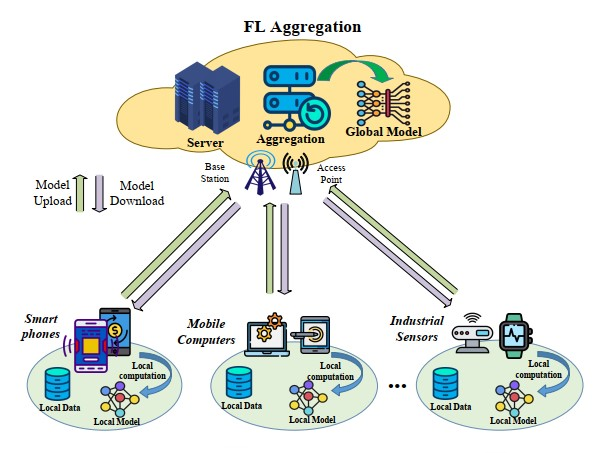
\includegraphics[height=8cm,width=10cm]{./arch/FL_architecture.jpg}
\caption[معماری یک شبکه یادگیری فدرال]{ معماری یک شبکه یادگیری فدرال\cite{a10}}
\label{wt}
\centering
\end{figure}

\section{پیشینه تحقیق}

پژوهشگران فعال در حوزه یادگیری فدرال در حال حاضر بیشتر بر دو چالش اصلی تمرکز دارند. اولاً، ناهمگونی داده در بین کارگران باعث کند شدن همگرایی مدل نسبت به یادگیری سنتی می‌شود. چالش دیگر هزینه ارتباطی در هر دو فرآیند بارگذاری و بارگیری مدل است که گلوگاه یادگیری توزیع شده است. به‌ خصوص در مورد سناریوهایی با تعداد دستگاه‌های زیاد در اینترنت اشیاء، این چالش جدی‌تر است. تعداد زیادی از کارها برای مقابله با این دو چالش پیشنهاد شده‌اند که می‌توان آن‌ها را در دسته‌بندی الگوریتم‌های بهینه‌سازی و استراتژی‌های کارآمد ارتباطات طبقه‌بندی نمود\cite{book_1}\cite{edge1}\cite{edge2}.

به عنوان مثال از الگوریتم‌های بهینه‌سازی می‌توان به انواع بهینه‌سازی‌های سراسری و محلی که سعی می‌کنند با استفاده از الگوریتم‌های مختلف، مانند گرادیان کاهشی، نمونه‌برداری تصادفی، گرادیان کاهشی تصادفی و غیره، به روزرسانی‌های مدل را در سرور مرکزی همگرا کنند. این روش‌ها برای کاهش هزینه ارتباطات و افزایش سرعت یادگیری مفید هستند. از طرف دیگر، می‌توان به استراتژی‌های کارآمدتر اشاره کرد که سعی می‌کنند با استفاده از روش‌های مختلف، مانند هماهنگ‌سازی دوره‌ای، هماهنگ‌سازی تصادفی، هماهنگ‌سازی بر اساس شرط و غیره، زمان و شرایط ارسال به روزرسانی‌های مدل را تعیین کنند. این روش‌ها برای حل مشکلات ناشی از نامتقارن بودن داده‌ها و نامتعادل بودن توزیع داده‌ها بین گره‌های محلی مناسب هستند. پژوهش‌های مختلف در این زمینه عموماً بر روی یک یا ترکیبی از چند از این روش‌ها تمرکز دارند.

\section{اهداف و دستاوردهای تحقیق}

باتوجه به اهمیت بارز روش‌های نوین یادگیری ماشین در دنیای امروزه و به خصوص کاربرد آن در اینترنت اشیاء، در این پروژه، سعی شده تا با استفاده از ظرفیت پردازش لبه یک چارچوب یادگیری فدرال مناسب که در آن چالش ارتباطات و ناهمگونی داده‌ها تا حد خوبی مدیریت شده ارائه دهد. شبیه‌سازی این نظریه در چارچوب نرم‌افزار‌های مطرح شبیه‌سازی از جمله \lr{GNS3}\LTRfootnote{Graphical Network Simulator-3} و \lr{Flower} و غیره انجام شده و نتایج نشان دهنده موثر بودن این راهکار است.

\section{ساختار گزارش}

در ادامه، فصل دوم مروری بر مفاهیم پایه مورد نیاز برای این پروژه را در بر میگیرد. فصل سوم به تعریف مسئله، معرفی و بررسی کامل مدل پیشنهادی برای حل مسئله، داده ها و چهارچوب کاری پروژه خواهد پرداخت. در نهایت، فصل چهارم ارزیابی و جمع بندی کلی پروژه را دربرمی‌گیرد.

% Chapter 2
\chapter{پیش زمینه و مروری بر مطالعات انجام شده}

رشد چشمگیر فناوری به همراه سهولت دسترسی به اینترنت در سال‌های اخیر باعث شده که بیشتر دستگاه‌های اطراف خود را متصل به اینترنت ببینیم. این دنیای جدید که به دنیای اینترنت اشیاء معروف است شامل خانه‌های هوشمند، دستگاه‌های پوشیدنی، خودروهای خودران و تلفن‌های هوشمند و... است که همگی زندگی روزمره انسان را تغییر داده‌اند. استفاده از این سیستم‌ها همگی باعث تولید حجم قابل توجهی داده در طول روز می‌شود که شرکت‌های بزرگ فناوری از این داده‌ها بهره برده و با استفاده از آن‌ها اقدام به انواع سرویس‌دهی به کاربران خود می‌نمایند\cite{b8}. شرکت‌های پیشرو برای تصمیم‌گیری‌های کلان مدیریتی و ارائه سرویس بهتر و با کیفیت‌تر به مشتریان، نیازمند استفاده از مدل‌های هوش‌مصنوعی برای ارتقاء کیفیت سیستم‌های هوشمند خود در جهت بهره‌برداری از این داده‌ها هستند. روش‌های متنوعی در رابطه با نحوه استفاده از این مدل‌ها وجود دارد. در ادامه روش‌های مختلفی از مطرح‌ترین روش‌ها توضیح داده می‌شود و نگاهی ریز بینانه‌تر به یادگیری فدرال و رابطه‌ آن با اینترنت اشیاء انداخته می‌شود\cite{ref5}.

\section{نگاه نزدیک‌تر به الگوریتم‌های یادگیری}

با توجه به رشد علم هوش مصنوعی و استفاده از روش‌های یادگیری ماشین، می‌توان از حجم بسیار زیاد داده تولید شده توسط گره‌های اینترنت اشیاء به نحو مطلوبی استفاده نمود و الگوریتم‌های مورد نظر، جهت رسیدن به اهداف مختلف را بر روی آن‌ها اجرا کرد. حال برای مدیریت و اجرای الگوریتم‌های یادگیری، روش‌های مختلفی وجود دارد که به توضیح هر یک از آن‌ها خواهیم پرداخت.

\subsection{یادگیری متمرکز}

این روش که در اکثر سیستم‌های حال حاضر امروزی مورد استفاده قرار می‌گیرد به این نحو است که تمام گره‌ها اطلاعات موجود خود را به صورت کامل به سیستم سرویس‌دهنده ابری ارسال می‌نمایند و سرویس‌دهنده ابری در حالی که تمام داده‌ها را در اختیار دارد، اقدام به اجرای الگوریتم‌های مورد نظر می‌کند. در شکل \ref{centralized} این روش به نمایش گذاشته شده است.

    \begin{figure}[H]
      \centering
      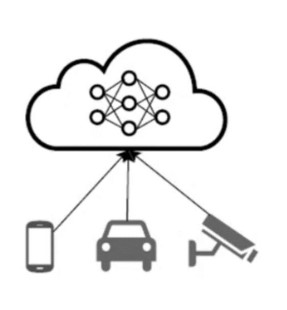
\includegraphics[height=4cm,width=6cm]{./types of ML/centralized .jpg}
      \caption[یادگیری متمرکز]{ یادگیری متمرکز\cite{ref6}}
      \label{centralized}
      \centering
    \end{figure}

سیستم‌های متمرکز تا پیش از این، اکثر نیازهای مربوطه را برطرف نموده‌اند ولی در دنیای امروزی و با توجه به زیاد شدن هر روزه دستگاه‌های متصل، موارد دیگری نیز مورد توجه واقع شده است. هزینه‌های ارتباطی ارسال حجم وسیع داده از یک سمت و نگرانی‌ها حول انتقال اطلاعات حساس و شخصی از سمت دیگر، توجه محققان را به سمت الگوریتم‌های غیر متمرکز و توزیع شده در یادگیری ماشین سوق داده است.

این روش دارای نقاط قوت و ضعف مختلفی است. از نقاط قوت این روش می‌توان به سرعت و دقت بالا، همگام‌سازی و یکنواختی داده‌ها و حفاظت و امنیت بالای داده‌ها اشاره کرد. از نقاط ضعف این روش می‌توان به وابستگی به هزینه و پایداری سرویس دهنده ابری، حساسیت به حجم و نوع داده‌های منتقل شده و چالش برانگیزی در برابر تغییرات محیط ذکر کرد. این روش در بسیاری از سرویس‌های آنلاین مورد استفاده قرار می‌گیرد.

\subsection{یادگیری غیرمتمرکز}

    در این روش هر گره به صورت مجزا اقدام به اجرای الگوریتم‌های مورد نظر می‌کند و در واقع پس از اجرای چند مرحله از کد، اطلاعات به‌روز شده را با گره‌های همسایه به اشتراک می‌گذارد. این کار به قدری ادامه پیدا می‌کند تا همگی به مقدار تعیین شده همگرا شوند. در شکل \ref{decentralized} این روش به نمایش گذاشته شده است.

    \begin{figure}[H]
      \centering
      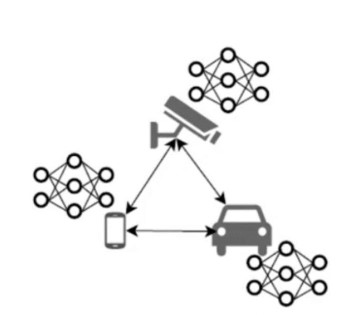
\includegraphics[height=4cm,width=6cm]{./types of ML/decentralized .jpg}
      \caption[یادگیری غیر متمرکز]{ یادگیری غیر متمرکز\cite{ref6}}
      \label{decentralized}
      \centering
    \end{figure}

 از مزایا و معایب این روش یادگیری این است که به گره‌ها اجازه می‌دهد که با توجه به شرایط و پارامتر‌های محلی خود، الگوریتم‌های خود را اجرا، تنظیم و بهینه‌سازی کنند. این روش همچنین باعث می‌شود که بار پردازشی و هزینه انتقال داده‌ها کاهش یابد و حریم خصوصی و حفاظت از داده‌ها حفظ شود. اما این روش نیز دارای چالش‌هایی است. از جمله سرعت و دقت پایین‌تر در پردازش داده‌ها، ناهمگام‌سازی و نامنظم بودن داده‌ها بین گره‌ها و نیاز به تضمین و تأیید صحت و کامل بودن داده‌ها. این روش در برخی از سیستم‌های آنلاین مانند بیت‌کوین\LTRfootnote{Bitcoin} و تورنت\LTRfootnote{Torrent} مورد استفاده قرار می‌گیرد.

\subsection{یادگیری توزیع شده}

    در این روش، مدیریت کل سیستم و تمام داده‌ها در اختیار یک هسته مرکزی قرار دارد ولی به دلیل نیاز به توان پردازشی بالا، این هسته بار پردازشی را بین گره‌های موجود تقسیم می‌کند. در ابتدای راه یادگیری توزیع شده، فرض بر این بوده است که تمام گره‌ها توان پردازشی یکسانی داشته و داده‌ها به میزان مساوی بین گره‌ها پخش خواهند شد. در شکل \ref{distributed} این روش به نمایش گذاشته شده است.

    \begin{figure}[H]
      \centering
      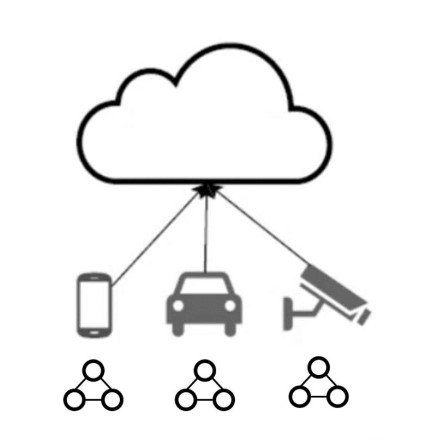
\includegraphics[height=4cm,width=6cm]{./types of ML/distributed .jpg}
      \caption[یادگیری توزیع شده]{ یادگیری توزیع شده\cite{ref6}}
      \label{distributed}
      \centering
    \end{figure}


\subsection{یادگیری فدرال}
    همان‌طور که در فصل اول اشاره شد، در یادگیری فدرال بر خلاف روش‌های متمرکز یادگیری ماشین، تحلیل داده‌ها به دستگاه‌های لبه، گره و یا سرور گیرنده منتقل می‌شود. یادگیری فدرال راه‌حلی مطلوب برای مدل‌سازی داده‌ها در تعداد زیادی دستگاه کارگر است. در این چارچوب، به جای ارسال داده‌های خام، پارامترهای مدل‌های محلی در هر گام آموزش به سرور منتقل می‌شود. در شکل \ref{federal} این روش به نمایش گذاشته شده است.
    سرور در حقیقت نقش رهبری را ایفا می‌کند و با توجه به نوع داده‌ها، یا مدل شبکه عصبی ایجاد کرده و آن را به سمت کاربران ارسال می‌کند. حال کاربران با توجه به داده‌های خود شبکه را آموزش می‌دهند و بعد از چند بار تکرار، وزن‌های به‌روزرسانی شده را به سمت سرور بر می‌گردانند. همان‌طور که در شکل \ref{federal} مشاهده می‌شود، داده‌ها همگی در سمت کاربر قرار گرفته‌اند و به سمت سرور ارسال نمی‌شوند. عدم ارسال بخش اطلاعات گره‌ها در یادگیری فدرال، حفظ حریم شخصی کاربران را ارتقا می‌بخشد.
    \begin{figure}[H] \centering
      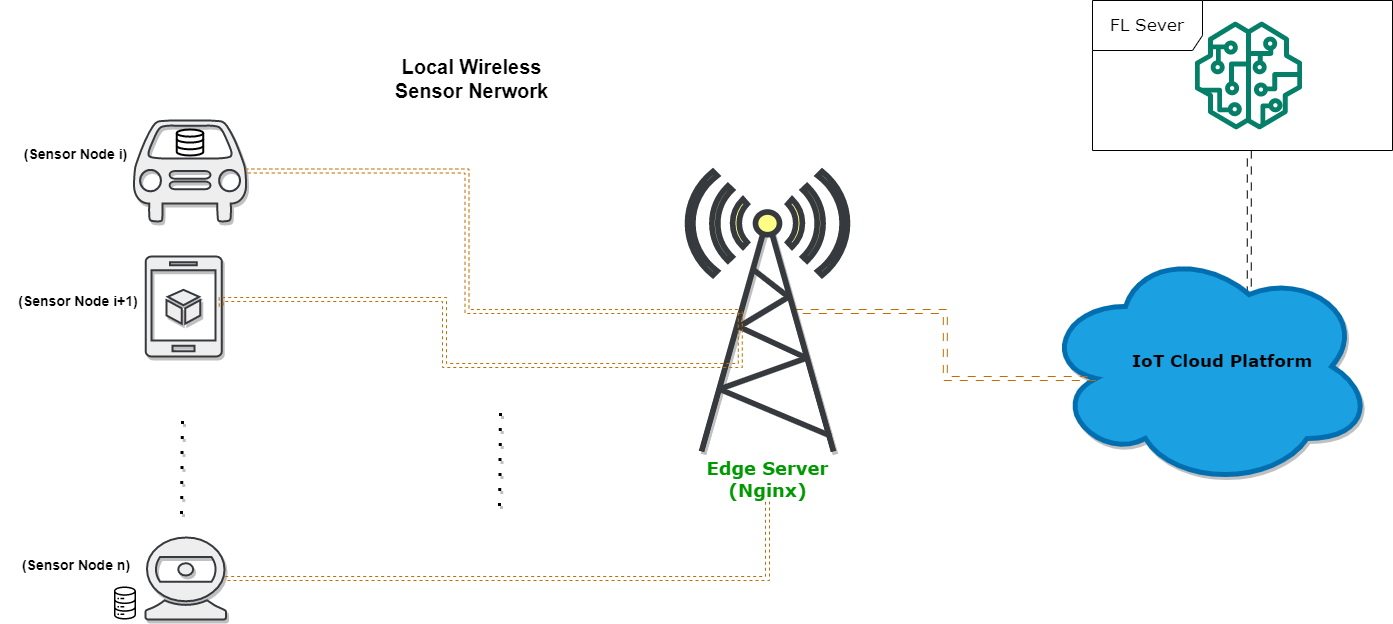
\includegraphics[height=8cm,width=15cm]{./IoT/State Diagram-Inter-connection.drawio.png}
      \caption{ شمایی از یادگیری فدرال در اینترنت اشیاء}
      \label{federal}
      \centering \end{figure}



      معمولاً برای تخمین و سنجش عملکرد روش‌های یادگیری ماشینی از مدل‌های شبکه عصبی استفاده می‌شود که کاربرد وسیعی در اکثر زمینه‌ها مانند پردازش تصویر، دسته بندی، پیش‌بینی و غیره دارند. امروزه با آمدن روش‌هایی آموزش و توسعه این روش‌ را از همیشه ساده‌تر شده است. علی‌رغم وجود مدل‌های گوناگون به عنوان مدل سراسری در یادگیری فدرال، اکثر استفاده‌های آن معطوف به مدل شبکه عصبی و به طور خاص‌تر شبکه‌های عصبی عمیق\LTRfootnote{Deep Neural Network} در پردازش تصویر به عنوان یکی از الزامات اساسی در اینترنت اشیاء می‌باشد. البته باید قبول کرد که در دسترس بودن و سادگی کار با آن‌ها نیز از دیگر عوامل روی‌ آوردن به آن‌ها می‌باشد. در ادامه به یکی از مطرح‌ترین استفاده از این مدل‌های دسته بندی کننده می‌پردازیم.



\subsection{الگوریتم FedAVG }

      از مطرح‌ترین و ساده‌ترین روش‌های ادغام کردن پارامتر‌های ارسالی (به عنوان مثال وزن‌ها و بایاس‌های شبکه عصبی) توسط تجمیع کننده الگوریتم میان‌گیری از آن‌ها با وزن یکسان بین تمامی کارگران می‌باشد. این الگوریتم با نام \lr{Federated Averaging} برای اولین بار در \cite{b6} مطرح شده است. در نسخه‌های اولیه یادگیری فدرال، این الگوریتم به صورت متمرکز درون تجمیع کننده در انتهای هر دور از یادگیری اجرا می‌شود تا در نهایت تمام کارگران با وزن یکسان در فرآیند یادگیری سهیم باشند. در ادامه شبه‌کد دو تکه اصلی مورد نیاز از اجرای این الگوریتم در تجمیع‌کننده و کارگران آورده شده است.
      
      
      از مهم‌ترین ایراداتی که می‌توان به این نوع الگوریتم گرفت این است که به علت ناهمگونی داده‌ها بین کارگران نباید در میانگین‌گیری وزن یکسانی به آنها داد. به همین دلیل طی سال‌های اخیرمدل‌های پیشرفته‌تری از این استراتژی معرفی شده است\cite{ref4}.
      
      
      \begin{algorithm}[H]
          \caption{بروزرسانی مشترک: اجرا در هر کارگر}
          \label{alg:client_update}
          \begin{algorithmic}[1]
              \State \textbf{ورودی:} بردار وزن مدل $w$، (\lr{Local Mini Batch})اندازه دسته‌های کوچک محلی $B$
              \State \textbf{خروجی:} بردار وزن مدل به‌روزشده $w'$
              
              \Function{بروزرسانی-مشترک}{$w, B$}
                  \State تقسیم $P_k$ به دسته‌هایی به اندازه $B$: $بچها \gets \text{تقسیم\_به\_بچها}(P_k, B)$
                  
                  \For{$i = 1$ تا $E$} \Comment{عبورهای آموزشی محلی}
                      \For{$هر دسته$ در $دسته‌ها$}
                          \State $w \gets w - \eta \cdot \nabla f(w,دسته)$ \Comment{بروزرسانی وزن‌های مدل}
                      \EndFor
                  \EndFor
                  
                  \State \Return $w$
              \EndFunction
          \end{algorithmic}
      \end{algorithm}
      
      \begin{algorithm}[H]
          \caption{میانگین‌گیری مشترک: اجرا در سرور}
          \label{alg:federated_averaging}
          \begin{algorithmic}[1]
              \State \textbf{ورودی:} نرخ یادگیری جهانی $\eta$، تعداد کارگر‌ها در هر دور $C$، تعداد عبور آموزشی محلی $E$، اندازه مینی‌بچ محلی $B$
              \State \textbf{خروجی:} بردار وزن مدل میانگین $w_{\text{avg}}$
              
              \Function{میانگین‌گیری-مشترک}{$\eta, C, E, B$}
                  \State مقداردهی اولیه بردار وزن مدل: $w \gets w_0$
                  
                  \For{$t = 1$ تا $\infty$} \Comment{دوره‌های آموزشی}
                      \State انتخاب به صورت تصادفی $C$ کارگر: $کارگر‌های\_انتخاب‌شده \gets \text{انتخاب\_کارگر‌ها}(C)$
                      
                      \For{$k$ در $کارگر‌های\_انتخاب‌شده$}
                          \State انجام بروزرسانی مشترک برای کارگر $k$: $w_k \gets \text{بروزرسانی-مشترک}(w, B)$
                          \State بروزرسانی بردار وزن مدل برای کارگر $k$: $w \gets \text{تجمیع\_وزن‌ها}(w, w_k)$
                      \EndFor
                      
                      \State محاسبه میانگین وزن‌های تمام کارگر‌ها: $w_{\text{avg}} \gets \text{محاسبه\_میانگین\_وزن‌ها}(w, C)$
                  \EndFor
                  
                  \State \Return $w_{\text{avg}}$
              \EndFunction
          \end{algorithmic}
      \end{algorithm}
      
\section{شبکه عصبی کانولوشنی}
مدل ‌کردن پردازش‌هایی که انسان قادر به انجام آن بر روی تصاویر است (برای مثال تشخیص هویت با استفاده از حس بینایی) با یک برنامه کامپیوتری از دستاورد‌های چندین ساله محققین حوزه تصویر بوده است. با معرفی بخش‌بندی معنایی\LTRfootnote{Semantic Segmentation } و شبکه‌های عمیق تصور شد که این مشکلات با استفاده از این روش جدید قابل حل‌شدن هستند. ولی مشکل بزرگ در مسیر استفادهٔ شبکه‌های عمیق برای پردازش تصاویر، هزینهٔ محاسبات این روش برای استفاده بر روی حجم زیاد داده‌ای که یک تصویر را تشکیل می‌دهد است. در حالت متداول شبکه‌های عمیق برای محاسبهٔ مقدار خروجی هر نورون، خروجی تمام نورون‌های لایهٔ قبل استفاده می‌شود و شیوهٔ استفاده از خروجی هر یک از نورون‌های قبل با یک پارامتر مشخص می‌شود. یک تصویر نمونه با تراکم پیکسلی نسبتاً کم، برای مثال 256 × 256 را می‌توان به صورت یک بردار به طول 65536 در نظر گرفت. باتوجه‌به نحوه پیچیدگی شبکه‌های عصبی عمیق می‌توان درک کرد که حرکت داده‌ای با این حجم در لایه‌های یک شبکه عمیق می‌تواند به چه اندازه از نظر محاسبات سخت و سنگین باشد.

\begin{figure}[H]
  \centering
  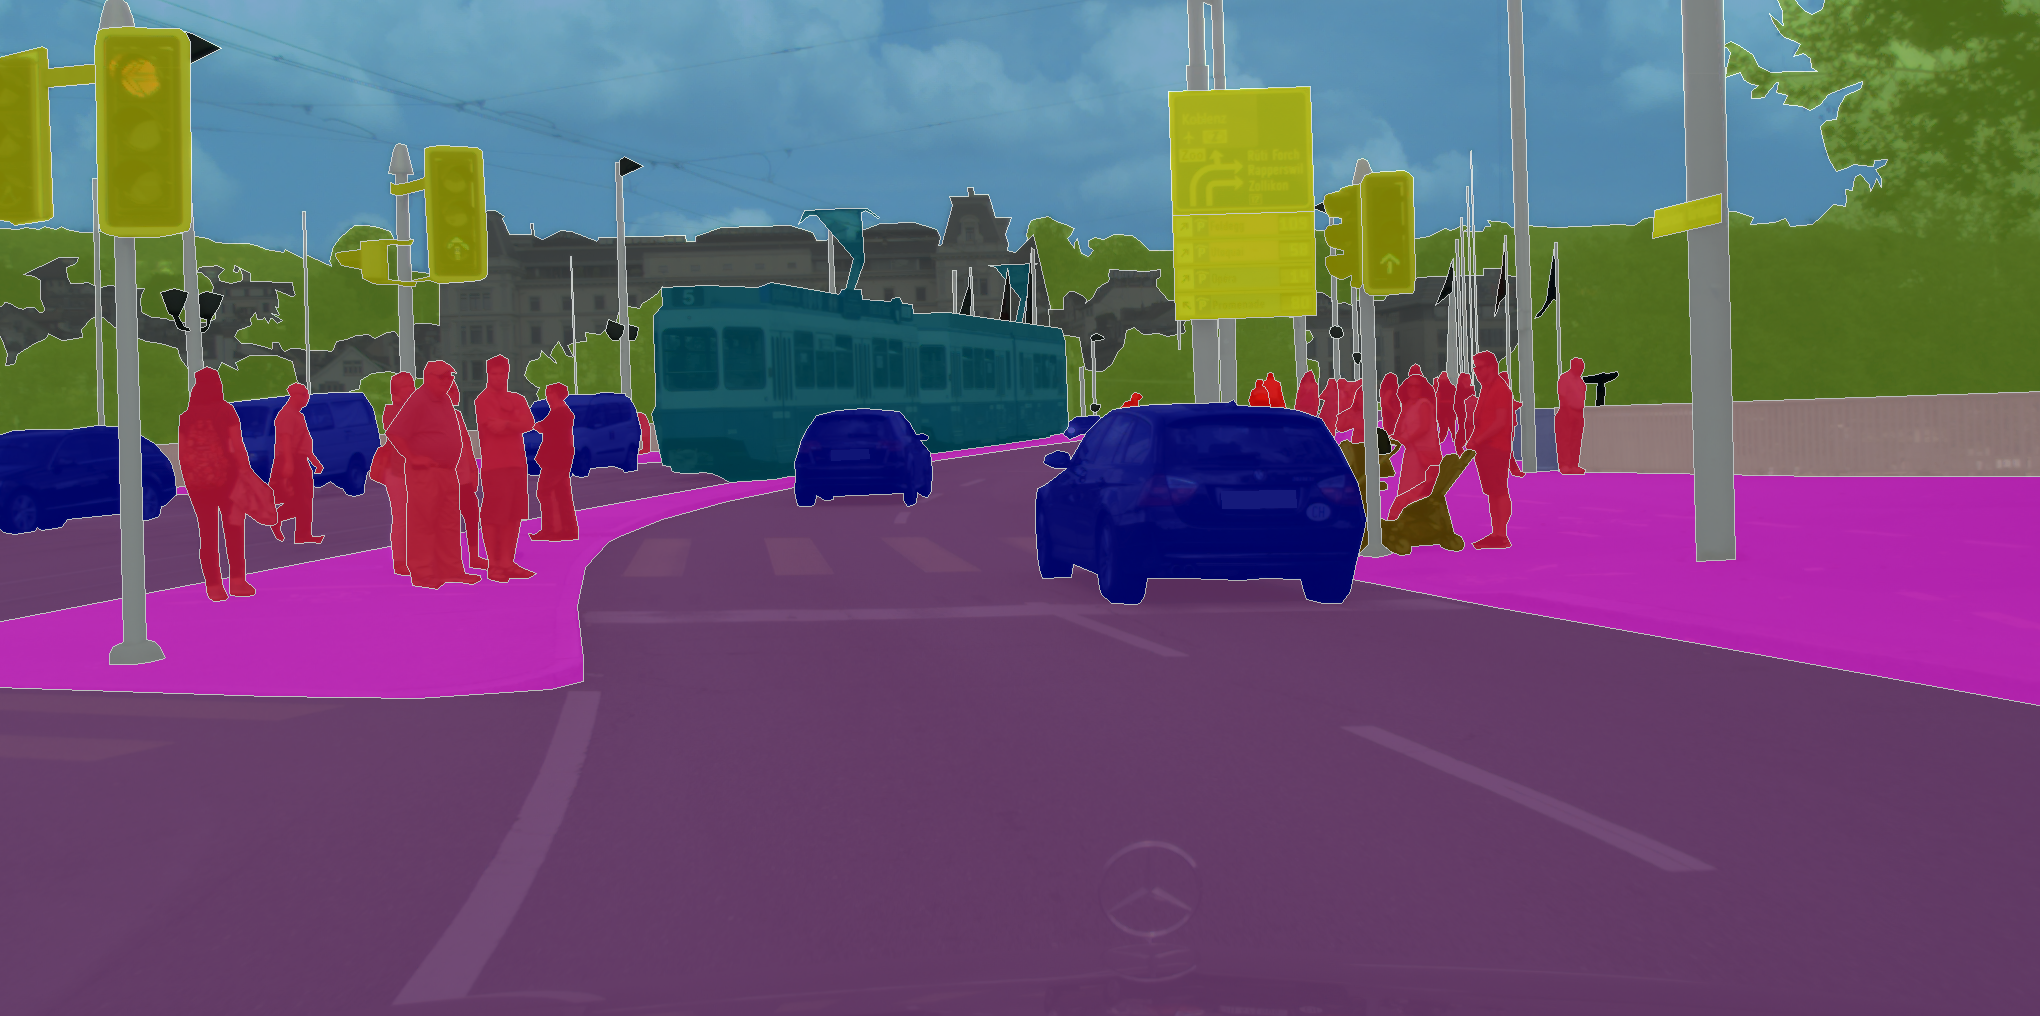
\includegraphics[height=8cm,width=12cm]{CNN/Zurich-Cityscapes.png}
  \caption[نمونه ی بخش بندی معنایی در ماشین های خودران]{ نمونه ی بخش بندی معنایی در ماشین های خودران\cite{ref7}}
  \label{CNN2}
  \centering
\end{figure}

برای عبور از این مانع، شبکه‌ای جدید با محوریت پردازش داده‌های تصویری (به‌ طورکلی تر پردازش سیگنال) طراح شد و این الگوریتم جدید را شبکه‌های عصبی کانولوشن\LTRfootnote{Convolutional Neural Networks } نام‌گذاری کردند. ایده اصلی این طرح جدید در این نکته بود که بهتر است برای محاسبهٔ خروجی هر نورون از خروجی تمام نورون‌های لایهٔ قبل استفاده نشود؛ بلکه کافی است فقط از همسایگان محدود از نورون‌های همسایه استفاده شود. در نتیجه هزینهٔ محاسبات برای پردازش و مهم‌تر از آن تعداد پارامترهای مدل کاهش می‌یابد. هر لایه از این شبکه (در ساده‌ترین حالت) با یک کرنل تعریف می‌شود که مقادیر آن به‌عنوان پارامترهایی قابل تغییر فرض می‌شود که شبکه در طول فرآیند یادگیری آنها را تنظیم می‌کند. ورودی هر لایهٔ تصویر (به‌عبارت ‌دیگر نقشهٔ ویژگی) و خروجی آن نیز به همین ترتیب است؛ ولی لزوماً رزولوشن این دو یکسان نیست. این کرنل بر روی تک‌تک پیکسل‌های تصویر اعمال می‌شود و تصویر خروجی تولید می‌شود. به این عملیات فیلتر کردن در شبکهٔ عصبی کانولوشن می‌گویند. در شکل \ref{CNN} معماری یک شبکه کانولوشن به عنوان نمونه آورده شده است.

\begin{figure}[H]
  \centering
  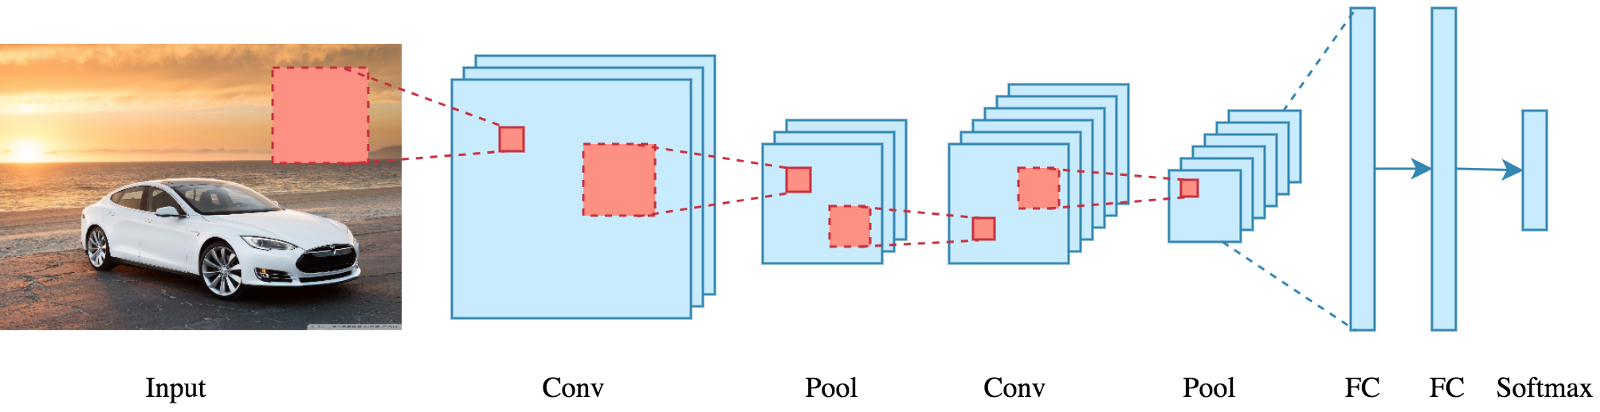
\includegraphics[height=5cm,width=15cm]{CNN/183560_qcMBDPuKpDvICcdd.png}
  \caption{ معماری یک شبکه کانولوشنی}
  \label{CNN}
  \centering
\end{figure}

این شبکه پس از معرفی توانست محبوبیت خاصی را بین محققان به دست آورد و همچنین مقدمه‌ای بر ساخت انواع پیشرفته‌تر از شبکه‌های عصبی برای عملیات مختلفی مانند تشخیص و شناسایی چهره\LTRfootnote{Face Recognition}، بخش‌بندی معنایی تصویر، تشخیص اشیاء، دسته‌بندی و گروه‌بندی تصاویر و غیره بشود.\cite{ref8}
\section{پردازش لبه}

در روش‌های مبتنی بر الگوی ابری، داده‌ها باید از طریق اینترنت برای یک مرکز داده متمرکز ارسال شود تا در آن‌جا پردازش شوند و نتیجه برای منبع بازگردانده شود. این روش برای حجم محدود و مشخصی از داده‌ها عملکرد خوبی دارد، اما هنگامی که حجم عظیمی از داده‌ها قرار باشد برای مراکز داده ارسال شود، در آن‌جا پردازش شود و نتیجه برای منبع بازگردانده شود مناسب نیست. زیرا نیاز به پهنای باند زیاد وجود دارد که مقرون‌به‌صرفه نیست. هم‌چنین مشکلات تاخیر و قطعی‌های غیرقابل پیش‌بینی شبکه، همگی می‌توانند باعث اختلال در عملکرد ارسال، دریافت و پردازش داده‌ها شوند. پژوهشگران برای حل این مشکل معماری پردازش لبه را ارائه کرده‌اند. پردازش لبه یک معماری توزیع‌شده است که در آن داده‌های کاربر در لبه شبکه و تا حد امکان نزدیک به دستگاه‌های انتهایی پردازش می‌شود. آمارها نشان می‌دهند که ساختار‌های مبتنی بر پردازش لبه در حال تغییر الگوی پردازش اطلاعات هستند و این احتمال وجود دارد که در آینده تغییرات مهمی در حوزه یادگیری به خصوص یادگیری‌های توزیع شده به وجود آورند\cite{edge1}.

در اصطلاح لبه شبکه به مکانی اشاره دارد که در آن داده‌ها تولید می‌شوند و تجهیزات محاسباتی در آنجا نصب شده‌اند. در محاسبات سنتی سازمانی، داده‌ها در سرورهای مرکزی ذخیره می‌شوند و از طریق شبکه محلی در اختیار کاربران قرار می‌گیرند. به عبارت دیگر، داده‌ها در زیرساخت‌های سازمانی ذخیره و پردازش شده و نتایج پردازش به کاربران ارسال می‌شود. این معماری بر اساس الگوی کلاینت و سرور است که بسیاری از برنامه‌های تجاری بر اساس آن عمل می‌کنند. با این حال، با پیدایش پردازش لبه، داده‌ها در نزدیک‌ترین مکان به منبع تولید آن‌ها پردازش شده و نتایج به کاربران ارسال می‌شود. این روش کمک می‌کند تا هزینه‌های ارتباطی کاهش یابد و حفظ حریم شخصی کاربران بهتر از قبل رعایت شود.

از آنجا که، تعداد دستگاه‌های متصل به اینترنت و حجم داده‌هایی که توسط دستگاه‌ها تولید می‌شوند و توسط کسب‌وکارها استفاده می‌شوند، فراتر از ظرفیت زیرساخت‌های مراکز داده سنتی است. یک مثال ساده در این زمینه، داده‌های تولیدشده در شبکه‌های اتومبیل‌های هوشمند است که به‌لحاظ تجاری و بازاریابی ارزش زیادی دارند و توسط خودرو تولید می‌شوند که عضو شبکه‌های اتومبیلی هستند. در سویی دیگر، داده‌های حساس‌به‌زمان وجود دارند که توسط تجهیزاتی مثل دوربین‌های نظارت تصویری ضبط می‌شوند و تصاویر از طریق اینترنت برای اپراتوری که مسئولیت نظارت بر دوربین‌ها را برعهده دارد ارسال می‌شود تا اگر مورد مشکوکی بود، اپراتور واکنش لازم را انجام دهد. در این روش نه‌تنها به پهنای باند زیادی برای ارسال داده‌ها نیاز است، بلکه باید اپراتور به‌سرعت به موارد مشکوک واکنش نشان دهد. حال اگر داده‌های تصویری به‌ شکل محلی توسط الگوریتم‌های هوشمند تحلیل شده و موارد مشکوک در قالب یک پیام متنی ساده برای اپراتور ارسال شود، به میزان قابل توجهی در پهنای باند صرفه‌جویی انجام می‌شود و زمان پاسخ‌گویی به رخدادها نیز کاهش پیدا می‌کند. در این حالت، فشار مضاعف بر اینترنت یا شبکه‌های گسترده وارد نمی‌شود و با مشکل ازدحام\LTRfootnote{Congestion} و اختلال\LTRfootnote{Disruption} روبه‌رو نخواهد شد.

\begin{figure}[H]
  \centering
  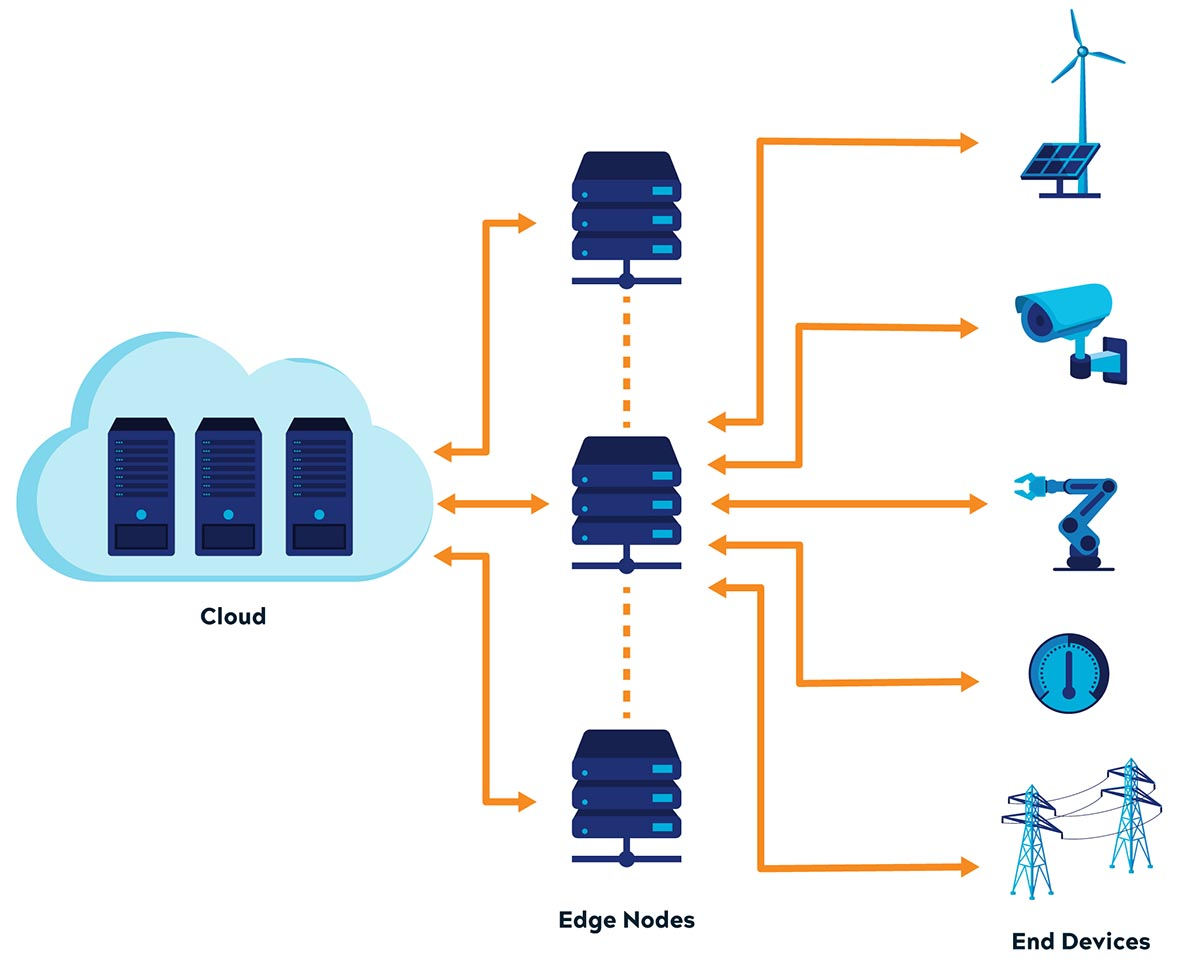
\includegraphics[height=8cm,width=13cm]{Edge/edge-computing-diagram.jpg}
  \caption{ دیاگرام یک شبکه دارای پردازش لبه}
  \label{Edge}
  \centering
\end{figure}

همین مسئله باعث شده تا معماران شبکه‌های کامپیوتری به‌جای طراحی مراکز داده متمرکز، به‌سراغ طراحی‌های مبتنی بر الگوی پردازش لبه بروند. به‌طوری‌که منابع ذخیره‌سازی و محاسباتی از مرکز داده به مکانی انتقال داده شود که نزدیک به منبع تولیدکننده داده‌ها است. دانستن این موضوع جالب خالی از لطف نیست که پردازش لبه بر مبنای یک تئوری خیلی ساده شکل گرفته است، اگر نمی‌توانید داده‌ها را به مرکز داده نزدیک کنید\cite{edge2}، مرکز داده را به داده‌ها نزدیک کنید.

\subsection{معماری‌های متنوع پردازش لبه}

همان‌طور که در شکل \ref{edge_arch} آمده است، می‌توان معماری‌های متنوعی برای حضور سرور لبه در شبکهٔ اینترنت اشیاء متصور شد. بسته به کاربرد و محل فیزیکی دستگاه‌ها می‌توان یکی از این معماری‌ها را برگزید. در این پروژه به دلیل ساده‌تر بودن و فراگیر بودن در کاربرد از معماری سلسله مراتبی استفاده شده است.

\begin{figure}[H]
  \centering
  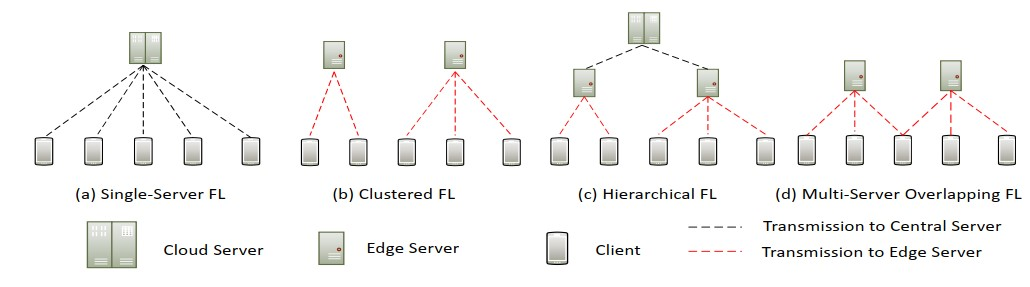
\includegraphics[height=7cm,width=15cm]{./arch/edge.jpg}
  \caption[انواع قرار گیری المان‌های اصلی در شبکه اینترنت اشیاء]{ انواع قرار گیری المان‌های اصلی در شبکه اینترنت اشیاء\cite{a10}}
  \label{edge_arch}
  \centering
\end{figure}

\section{یادگیری فدرال در اینترنت اشیاء}

شبکه‌های نوظهور اینترنت اشیا همچون دستگاه‌های پوشیدنی، خودروهای خودران یا خانه‌های هوشمند شامل تعداد بسیار زیادی حسگر هستند. این حسگرها توانایی جمع‌آوری عکس‌العمل و سازگاری با داده‌ها برای کاربرد بی‌درنگ را برای دستگاه‌های اینترنت اشیا فراهم می‌سازند. به عنوان مثال، خودروهای خودران به منظور عملکرد صحیح نیازمند یک مدل به روز از ترافیک شهری، اماکن و رفتار افراد پیاده هستند که این داده‌ها را از حسگرها دریافت می‌کند. ساخت مدلی سراسری در این حوزه به دلیل عدم تمایل افراد به در اختیار گذاشتن اطلاعات فردی، مانند اطلاعات مکانی و محدودیت در ارتباطات هر دستگاه بسیار مشکل است. از این رو، روش‌های یادگیری فدرال می‌توانند مدلی سازگار با تغییرات ایجاد نمایند و این سیستم‌ها را در عین حفظ حریم شخصی به خوبی آموزش دهند. شکل \ref{iot} بیانگر تنها بخشی از حوزه‌هایی است که در آینده‌ای نه چندان دور از ترکیب این دو حوزه به وجود می‌آید.
\begin{figure}[H]
  \centering
  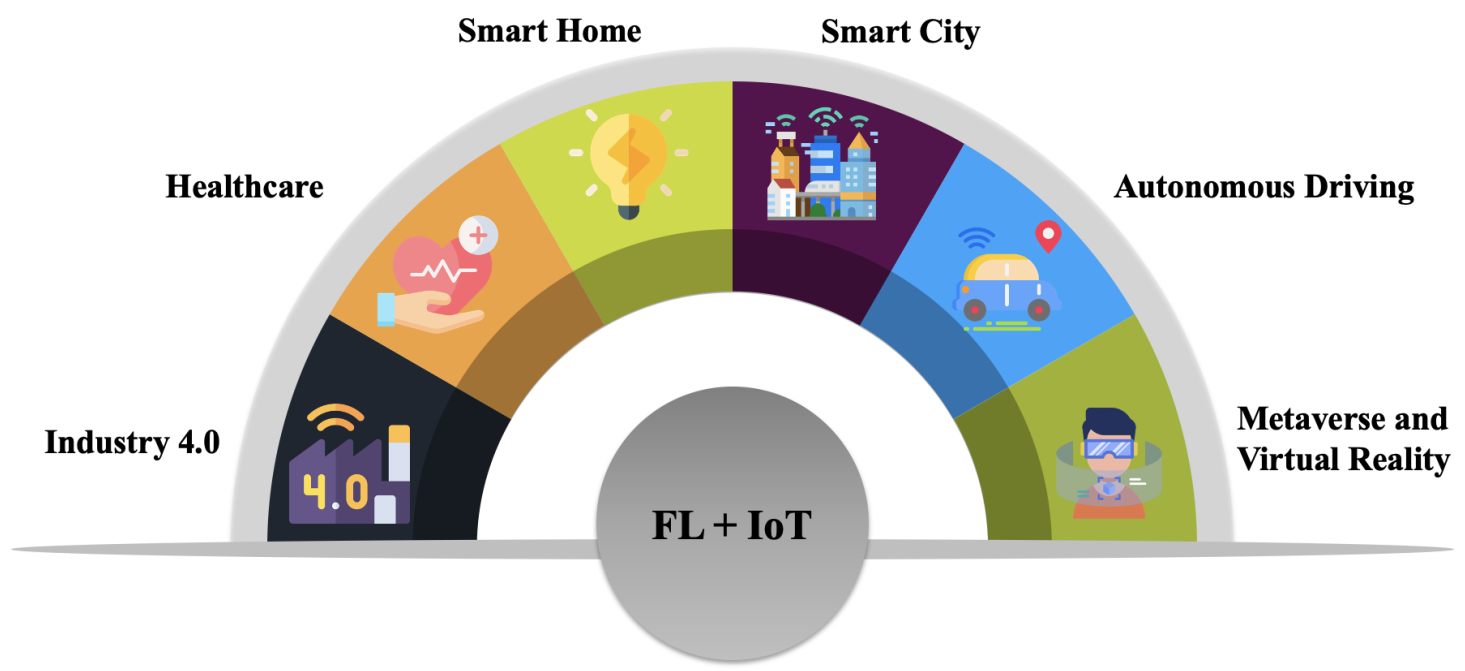
\includegraphics[height=7cm,width=13cm]{./IoT/IOT.png}
  \caption[کاربرد‌های یادگیری فدرال در اینترنت اشیاء]{ کاربرد‌های یادگیری فدرال در اینترنت اشیاء\cite{a10}}
  \label{iot}
  \centering
\end{figure}

\section{جمع بندی}
ایجاد بستری که تمامی موارد بالا در آن نقش پررنگی ایفا می‌کنند، می‌تواند محیط خوبی برای توسعه برنامه‌های مختلف با توجه به نیازهای کاربر باشد. این پروژه تنها بخشی از این نیاز‌ها را پوشش می‌دهد که کاربرد نسبتاً بالایی در دسته‌بندی تصاویر را ارائه می‌کند. در اینجا، سعی می‌شود با استفاده از ساده‌سازی‌های صورت گرفته، به تأکید بر پیاده‌سازی سیستمی که از یادگیری فدرال بهره می‌برد پرداخته شود. در نهایت با توجه دانش قبلی در مورد موارد ذکر شده در این فصل و بهره‌گیری از شبیه‌سازی‌های متنوع، به دسته‌بندی داده‌های مجموعه داده CIFAR-10 با استفاده از یک شبکه عصبی کانولوشن روی یک بستر شبکه اینترنت اشیاء که در آن از پردازش لبه استفاده شده خواهیم پرداخت. در فصل بعدی به جزئیات بیشتر این شبیه‌سازی پرداخته می‌شود.
%%%%%%%%%%%%%%%%%%%%%%%%%%%%%

% Chapter 3

\chapter{چارچوب کاری پروژه}

این فصل به معرفی داده‌های مسئله و همچنین معرفی و بررسی کامل مدل پیشنهادی مبتنی بر معماری شبکه عصبی کانولوشن می‌پردازد. مضاف بر این، چارچوب\LTRfootnote{Framework} استفاده شده و محیط شبیه‌سازی نیز مورد بحث قرار می‌گیرد.

\section{مجموعه داده تعریف شده در مسئله}

این بخش، به بررسی داده‌های مورد استفاده در آموزش شبکه‌های عصبی و مدل پیشنهادی برای حل مسئله می‌پردازد. این داده‌ها و مدل پیشنهادی برای حل مسئله، بر اساس مجموعه‌داده CIFAR-10 و کتابخانه PyTorch تعریف شده‌اند.
مجموعه‌داده CIFAR-10 شامل 60,000 تصویر رنگی ۳۲ در ۳۲ پیکسل  در 10 کلاس مختلف با 6000 تصویر در هر کلاس است. این کلاس‌ها شامل هواپیما، اتومبیل، پرنده، گربه، گوزن، سگ، قورباغه، اسب، کشتی و کامیون هستند. از این تعداد تصاویر، 50,000 تصویر برای آموزش و 10,000 تصویر برای تست استفاده می‌شود. شکل \ref{cifar} نمایی از این کلاس‌ها را نشان داده است.

\begin{figure}[H]
    \centering
   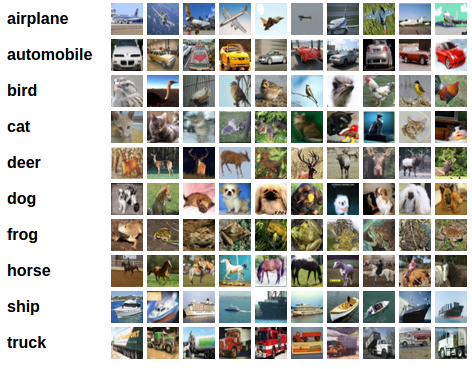
\includegraphics[height=10cm,width=12cm]{./cifar/cifar10.png}
   \caption{ نمونه‌ای از تصاویر دیتاست CIFAR10}
   \label{cifar}
   \centering
\end{figure}


برای آموزش شبکه عصبی، از کتابخانه PyTorch استفاده می شود. PyTorch یک کتابخانه یادگیری عمیق با قابلیت های بالا برای آموزش شبکه های عصبی است. در این پروژه، یک شبکه عصبی کانولوشنی تعریف شده و با استفاده از داده های آموزش CIFAR-10 آموزش دیده است. 
برای تعریف شبکه عصبی و آموزش آن، از تابع هزینه CrossEntropyLoss و الگوریتم بهینه سازی نزول گرادیان تصادفی\LTRfootnote{Stochastic Gradient Decent } با نرخ یادگیری \lr{0.001} استفاده شده است. تابع هزینه CrossEntropyLoss یک تابع هزینه مناسب برای مسائل طبقه بندی چند کلاسه است.


\section{مدل استفاده شده برای حل مسئله}

این مسئله از یک شبکه عصبی کانولوشن نسبتاً ساده بهره می‌گیرد. تابع فعال‌ساز\LTRfootnote{Activation Funcion} استفاده شده در هر لایه آن ReLU است که باعث پایداری شبکه می‌شود و رفتار خطی از خودش نشان می‌دهد.
شبکه دارای دو لایه کانولوشن و سه لایه تماماً متصل\LTRfootnote{Fully Connected Layar} است. در هر لایه کانولوشن، از یک لایه MaxPool2d برای کاهش ابعاد ویژگی‌ها استفاده می‌شود. سپس در هر مرحله ویژگی‌های سطح بالاتر استخراج می‌شوند تا نوبت به لایه‌های مخصوص به دسته‌بندی برسد. در نهایت بعد از استخراج ویژگی‌های منحصر به فرد هر تصویر و پیدا شدن مقدار احتمال حضور در هر یک از دسته‌ها، خروجی از طریق سه لایه تماماً متصل به یک بردار با ۱۰ عنصر تبدیل می‌شود که نشان‌دهنده احتمالات دسته‌بندی مختلف برای هر یک از کلاس‌های مجموعه داده است. نمودار مربوط به این شبکه در شکل \ref{CNN3} قابل مشاهده است.


\begin{figure}[h]
\usetikzlibrary{positioning, fit}
\resizebox{1\textwidth}{!}{%
\begin{tikzpicture}[x=2.5cm, y=2.5cm, >=stealth, every node/.style={minimum size=4.5cm,font=\fontsize{50}{66}\selectfont\bfseries}]
   
        % nodes
\node [draw] (input) at (0,0) {\lr{Input (32x32x3)}};
\node [draw, right=of input] (conv1) {\lr{Conv2d(3, 6, 5)}};
\node [draw, right=of conv1] (relu1) {\lr{ReLU}};
\node [draw, right=of relu1] (pool1) {\lr{MaxPool2d(2, 2)}};
\node [draw, below=of pool1] (conv2) {\lr{Conv2d(6, 16, 5)}};
\node [draw, right=of conv2] (relu2) {\lr{ReLU}};
\node [draw, right=of relu2] (pool2) {\lr{MaxPool2d(2, 2)}};
\node [draw, below=of pool2] (fc1) {\lr{Linear(16x5x5, 120)}};
\node [draw, right=of fc1] (relu3) {\lr{ReLU}};
\node [draw, right=of relu3] (fc2) {\lr{Linear(120, 84)}};
\node [draw, right=of fc2] (relu4) {\lr{ReLU}};
\node [draw, below=of relu4] (fc3) {\lr{Linear(84, 10)}};
\node [draw, right=of fc3] (output) {\lr{Output}};

% arrows
\draw [->, line width=2mm] (input) -- (conv1);
\draw [->, line width=2mm] (conv1) -- (relu1);
\draw [->, line width=2mm] (relu1) -- (pool1);
\draw [->, line width=2mm] (pool1) -- (conv2);
\draw [->, line width=2mm] (conv2) -- (relu2);
\draw [->, line width=2mm] (relu2) -- (pool2);
\draw [->, line width=2mm] (pool2) -- (fc1);
\draw [->, line width=2mm] (fc1) -- (relu3);
\draw [->, line width=2mm] (relu3) -- (fc2);
\draw [->, line width=2mm] (fc2) -- (relu4);
\draw [->, line width=2mm] (relu4) -- (fc3);
\draw [->, line width=2mm] (fc3) -- (output);

\end{tikzpicture}
}
\caption{ساختار شبکه عصبی کانولوشن استفاده شده در مسئله ۱۰ کلاسه}
\label{CNN3}
\end{figure}
برای بهبود عملکرد شبکه، می‌توان از روش‌های مختلفی استفاده کرد. برای مثال، می‌توان تعداد فیلتر‌ها در لایه‌های کانولوشن را افزایش داد، یا از روش‌های منظم‌سازی مانند Dropout یا \lr{Batch Normalization} استفاده کرد. همچنین، می‌توان تابع فعال‌ساز ReLU را با توابع فعال‌ساز دیگری مانند LeakyReLU یا Sigmoid جایگزین کرد. در نهایت، میتوان شبکه را با داده‌های آموزش بسیار بیشتر و با استفاده از روش‌های بهینه‌سازی پیشرفته‌تر آموزش داد.

\section{محیط توسعه استفاده شده }

محیط‌های توسعه متعددی برای پیاده‌سازی سناریوهای مختلف تولید شده‌ است. به عنوان مثال در تراز صنعتی، چارچوب \lr{FATE} توسط محققین شرکت \lr{Facebook} توسعه پیدا کرده است\cite{a1}. نقطه قوت این محصول امنیت و ایمنی بالا و قابل اطمینان برای کاربردهای کلان صنعتی می‌باشد. محیط دیگری که برای کاربردهای عملی و سهولت در استفاده توسط مهندسین آلمانی توسعه یافته است، \lr{Flower} نام دارد\cite{b1}. 

\lr{FATE} و \lr{Flower} هر دو چارچوب‌های منبع‌باز\LTRfootnote{Open Source} هستند که به توسعه‌دهندگان اجازه می‌دهند سناریوهای گوناگون یادگیری فدرال را پیاده سازی کنند. \lr{FATE} روی فراهم آوردن چارچوب محاسبات امن برای پشتیبانی از اکوسیستم هوش مصنوعی فدرال تمرکز دارد، در حالی که \lr{Flower} در هدف فراهم آوردن رویکردی کاربرپسند به یادگیری فدرال که با هر چارچوب یادگیری ماشین و زبان برنامه نویسی سازگار است، قرار دارد. هر دوی این محیط‌ها ویژگی‌ها و قابلیت‌های منحصر به فرد خود را دارند، به طوری که توسعه دهندگان می توانند از بین این دو یکی را که بهترین گزینه برای نیاز‌های آن‌ها است، انتخاب کنند. در این پروژه به دلیل سهولت دسترسی و دسترسی در محیط‌های شبیه‌سازی مختلف و فراهم بودن مثال‌های متعدد از سناریو‌های پیش‌فرض از این محیط به عنوان ابزاری برای پیاده‌سازی یادگیری فدرال در اینترنت اشیاء استفاده شده است. قابل ذکر است که این محیط نیازهای مربوط به پیاده‌سازی شرایط متنوع را به خوبی برطرف می‌سازد. از ویژگی‌های بارز این محیط می‌توان به سازگاری کامل با کتابخانه‌ها و محیط‌های دیگر توسعه یادگیری ماشین و هوش مصنوعی از جمله \lr{Pytorch} و \lr{Tensorflow} اشاره نمود.

\begin{figure}[H]
    \centering
   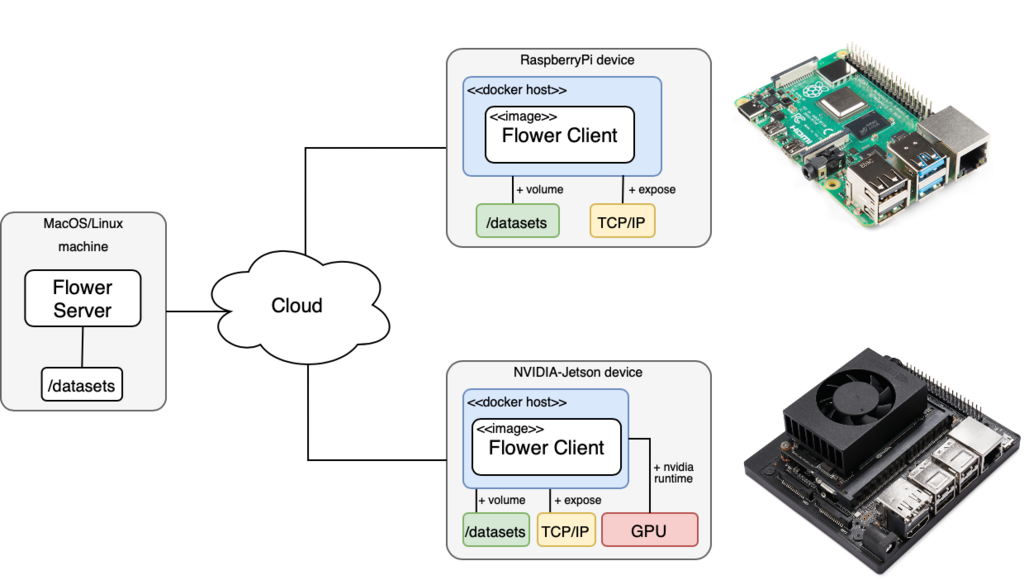
\includegraphics[height=8cm,width=10cm]{./Embedded/demo_diagram.png}
   \caption{ نمونه‌ای از پیاده سازی یادگیری فدرال روی دستگاه‌های تعبیه شده}
   \label{ pii }
   \centering
\end{figure}

برای پیاده‌سازی سرور لبه در دنیای واقعی نیز، مشابه سرور عمل می‌شود با این تفاوت که توان پردازشی می‌تواند تا حد امکان به اندازه‌ای که وقفه‌ای در مرحله یادگیری و آزمون صورت نگیرد، ساده‌تر در نظر گرفته شود.  الزاماً فرض بر این است که سرور لبه و سرور تجمیع‌کننده هر دو همیشه در شبکه فعال هستند و دائماً در حال گوش دادن روی یک پورت خاص به کارگران درخواست‌دهنده هستند. از طرف دیگر، کارگران که دستگاه‌های انتهایی هستند، می‌توانند با توجه به ماهیت کم‌توان بودن برای مصرف بهینه انرژی، به خواب‌های عمیق یا کوتاه‌مدت بروند. در عین حال سرور لبه می‌تواند به جای آن‌ها پاسخگوی سرور تجمیع‌کننده باشد تا گره دستگاه کم‌توان مجدداً به شبکه اضافه شود و پارامتر‌های خود را ارسال کند.

\section{پروتکل‌های انتقال داده در شبکه}

تقریباً تمامی چارچوبهای یادگیری فدرال از پروتکل امن\lr{gRPC}\LTRfootnote{gRPC Remote Procedure Calls} استفاده می‌کنند. \lr{gRPC} یک چارچوب متن‌باز و پر قدرت برای تماس‌های رویه‌ای از راه دور (RPC) است که توسط گوگل ایجاد شده است. این چارچوب قابلیت اجرا در هر محیطی را دارد و می‌تواند به طور کارآمد خدمات را درون و بین مراکز داده با پشتیبانی قابل‌تعویض برای توازن بار، ردیابی، بررسی سلامت و احراز هویت متصل کند. در این پروژه برای پردازش لبه از سرویس قدرتمند \lr{Nginx} استفاده شده است تا بتواند خواسته‌های مربوط به Proxy سرور را در لبه شبکه پوشش دهد.
از قابلیت‌های پیش‌فرض پلتفرم nginx پشتیبانی از این پروتکل است. همان‌طور که در شکل \ref{ grpc } نشان داده شده این پلتفرم می‌تواند به خوبی بسته‌\LTRfootnote{Packet}های grpc را انتقال بدهد. اما نکته حائز اهمیت آن است که ساختار بسته‌های grpc باید در هر دو طرف کلاینت و سرور کاملاً مشخص شده باشد (اصطلاحاً \lr{protobuf}). از آن‌جایی که nginx فاقد ساختار هر بسته است، تنها می‌تواند با استفاده از مشخصات داخل هدر فایل، اقدام به ارسال بسته کند. به عبارت دیگر، نمی‌توان به اطلاعات داخل بسته‌ها در وسط راه دسترسی پیدا کرد. البته از آن‌جایی که به صورت پیش‌فرض از این نوع بسته پشتیبانی می‌کند، قابلیت‌های خوبی در رابطه با مدیریت این نوع بسته قرار می‌دهد؛ مانند تعادل بار\LTRfootnote{Load Balancing} هنگام کار با چندین سرور به صورت همزمان و فشرده‌سازی\LTRfootnote{Compression} بسته‌های رد و بدل شده در شبکه.

\begin{figure}[H]
    \centering
   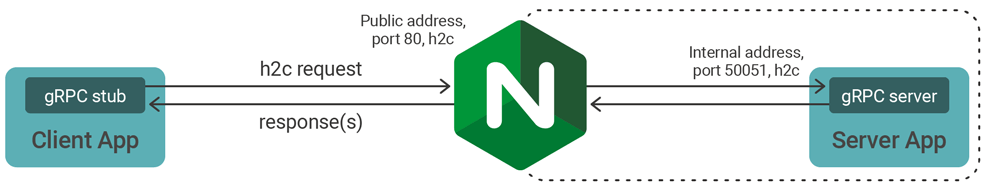
\includegraphics[height=4cm,width=14cm]{./GRPC/gRPC-nginx-proxy.png}
   \caption{ استفاده از nginx به عنوان پروکسی سرور}
   \label{ grpc }
   \centering
\end{figure}

میدانیم که nginx به خودی خود یک proxy server میباشد که در نگاه بالاتر با داشتن یک سرور لبه از نوع grpc میتوانیم به مراتب عملیات بیشتری در شبکه انجام بدهیم و با داشتن دیتای ارسالی کلاینت و سرور در لبه، در جدیدی از  قابلیت‌ها به روی مان باز خواهد شد.

\section{محیط شبیه‌سازی پیاده شده}

برای پیاده‌سازی سناریو ذکر شده از محیط قدرتمند شبیه‌سازی \lr{GNS3} استفاده شده است. در این محیط از دستگاه‌هایی با توان پردازشی محدود به‌عنوان کارگر و یک سرور مرکزی به‌عنوان تجمیع‌کننده استفاده شده است. همچنین از دستگاه‌هایی با توان پردازشی کمتر از سرور اصلی تجمیع‌کننده اما بیشتر از کارگران به‌عنوان مرکز پردازشی لبه استفاده شده است. شبکه داخلی حاوی سرور اصلی، کارگران و سرور لبه به‌عنوان یک شبکه اینترنت اشیاء مستقل که میتواند از پروتکل‌های مطرح شبکه‌های سنسوری بی‌سیم مثل بلوتوث مش\LTRfootnote{Bluetooth Mesh Sensor Networking} یا LORA\LTRfootnote{Long Range Wide Area} استفاده کند، پشت یک NAT\LTRfootnote{Network Address Translation} قرار دارد. تمامی این شبیه‌سازی‌ها بر روی یک لپ‌تاپ با ۱۶ گیگابایت رم و پردازنده ۸ هسته‌ای \lr{intel core i7} با فرکانس کاری ۳.۳ گیگاهرتز اجرا شده است. شکل \ref{scheme} بیانگر تصویری از این شبیه‌سازی می‌باشد.

\begin{figure}[H]
    \centering
   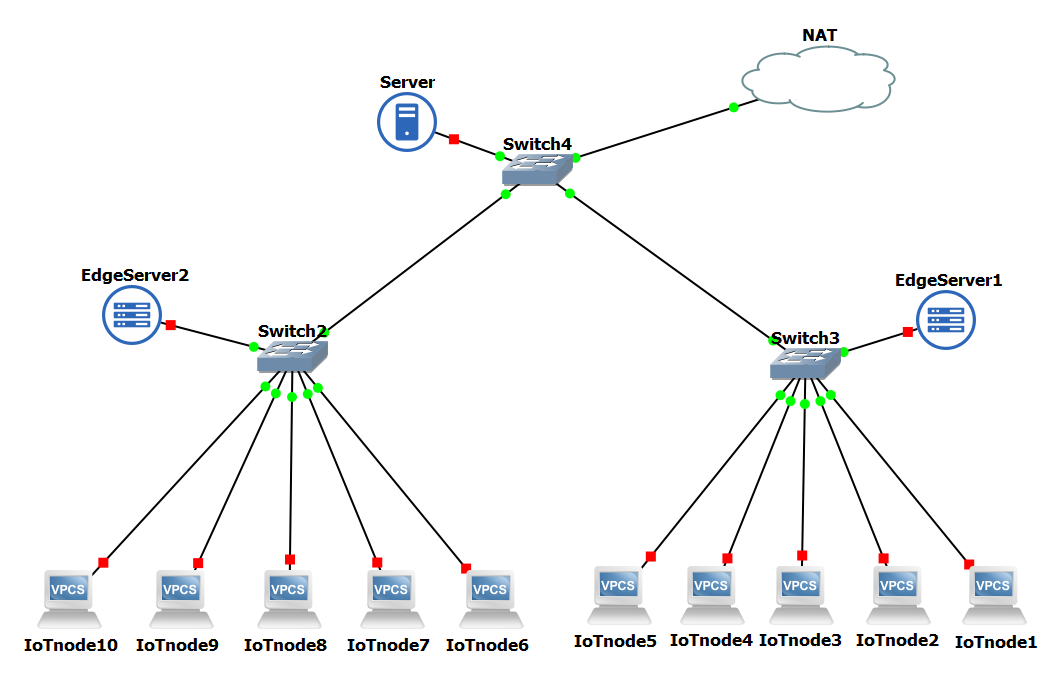
\includegraphics[height=8cm,width=14cm]{./GNS3/scheme.png}
   \caption{ محیط شبیه‌سازی شده در محیط نرم‌افزار \lr{GNS3}}
   \label{scheme}
   \centering
\end{figure}

\begin{figure}[H]
    \centering
   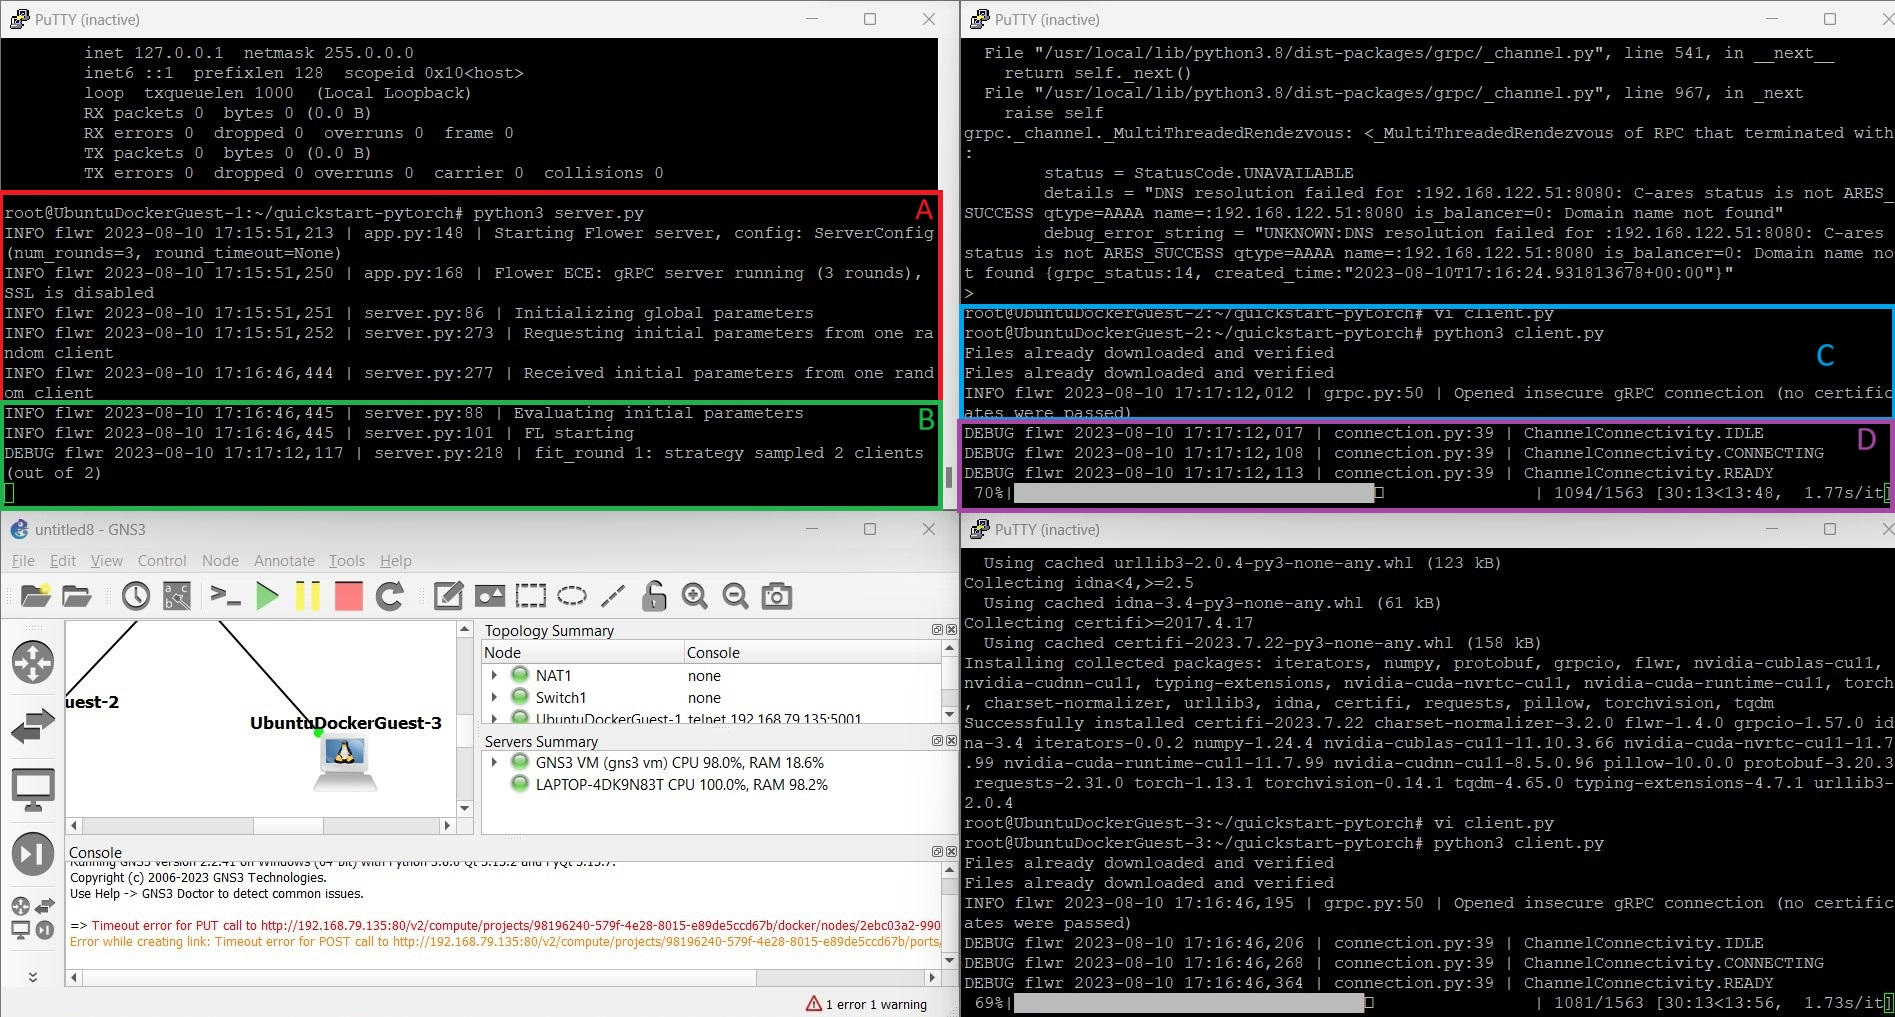
\includegraphics[height=12cm,width=16cm]{./GNS3/running.jpg}
   \caption{ نمونه‌ای از اجرای فرایند یادگیری و تست توسط یک شبکه ساده دارای دو کارگر}
   \label{running}
   \centering
\end{figure}


باتوجه به‌ شکل \ref{running}، قسمت‌های A و B مخصوص ترمینال سرور اصلی هستند و C و D نیز برای یکی از کارگران آورده شده‌اند. در ابتدا با اجرا شدن قسمت \lr{A}، سرور شروع به گوش دادن روی پورت و آدرس داده ‌شده (در اینجا آی‌پی آدرس سرور هاست در شبکه داخلی و روی یکی از پورت‌های آزاد معمولاً ۸۰۸۰) سپس منتظر می‌ماند تا تعدادی کارگر که حداقل آنها از قبل در کد برنامه تعریف شده به سرور وصل بشوند. سپس با رسیدن این تعداد به حداقل، فرآیند یادگیری آغاز می‌شود. وزن‌ها و بایاس‌های شبکه عصبی نیز در ابتدا در دور صفر از یکی از کارگران به صورت تصادفی دریافت می‌شوند (معمولاً اولین کارگری که وصل می‌شود). 
در کارگران نیز ابتدا با اجرا شدن کد برنامه در محیط سیستم عامل (در اینجا \lr{Ubunto})، ابتدا اقدام به دریافت فایل‌های مجموعه داده می‌کند که در اینجا از داده‌های CIFAR-10 استفاده شده است. پس از مبادرت به چک‌های اولیه از لحاظ معتبر بودن مجموعه داده و پیش‌نیاز‌های لازم، نوبت به ساخت کانال امن با استفاده از پروتکل GRPC می‌باشد. پس از رد و بدل کردن پیام‌های اولیه بر بستر \lr{HTTP2}، کانالی منحصر به فرد بین این کارگر و سرور اصلی ایجاد شده و تا پایان یادگیری باز می‌ماند. سپس بعد از وصل شدن کارگرهای بعدی به همین منوال، فرآیند در تمامی دستگا‌ه‌ها شروع می‌شود.

\begin{figure}[H]
    \centering
   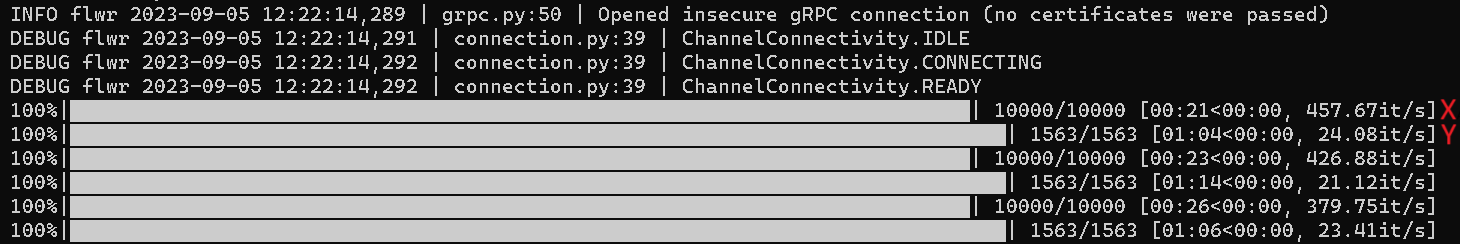
\includegraphics[height=4cm,width=16cm]{./simulations/client.png}
   \caption{ نمونه‌ای از کنسول یک کارگر در حال اجرای یادگیری فدرال}
   \label{client}
   \centering
\end{figure}


شکل \ref{client} نمونه‌ای از این فرآیند را در هر دور در هر کارگر با جزئیات بیشتری نشان می‌دهد. همان‌طور که مشخص است، مجموعه داده‌ CIFAR-10 شامل ۵۰ هزار تصویر آموزش و ۱۰ هزار تصویر تست است که باید توجه داشتیم که همان‌طور که از روی شکل شبیه‌سازی پیدا است، قسمت X بیانگر مرحله تست روی ۱۰ هزار عکس و مرحله Y بیانگر آموزش روی ۵۰ هزار تصویر این مجموعه داده می‌باشد. نکته قابل توجه این است که با توجه به اینکه اندازه هر batch برابر با ۳۲ است، با تقسیم ۵۰ هزار تصویر به ۱۵۳۲ دسته ۳۲تایی می‌رسیم تا در فرآیند آموزش از آن استفاده شود.

نکته دیگر مورد اهمیت این است که همان‌طور که توقع داریم، سرعت فرآیند آموزش به دلیل به‌روزرسانی شدن وزن‌ها در مدل از  فرآیند تست سریع تست و آخرین المان از هر خط  که به صورت تعداد عملیات بر ثانیه\LTRfootnote{Iteration Per Second} آمده است قرار دارد، با توجه به محدود بودن سخت‌افزاری در سیستم‌های اینترنت اشیاء، همان‌طور که از شکل \ref{running} واضح است، گاهاً این سرعت تا ۱ عملیات بر ثانیه کاهش پیدا می‌کند که این خود نشانی از اهمیت آن به عنوان گلوگاه اصلی در یادگیری فدرال در شبکه‌هایی با منابع محدود است.



%%%%%%%%%%%%%%%%%%%%%%%%%%%%%

% Chapter 4
\chapter{نتیجه‌گیری و پیشنهادها}


در این فصل، به ارزیابی مدل در برابر معیارهای مختلف پرداخته می‌شود و دقت‌ به دست آمده توسط مدل روی داده‌های تست گزارش می‌شود. لازم به ذکر است همان‌طور که گفته شد، در هر دور از یادگیری فدرال، ۵۰۰۰۰ تصویر برای آموزش و ۱۰۰۰۰ تصویر برای ارزیابی در نظر گرفته شده است.

\section{معرفی معیارهای مختلف}

شاخص‌های ارزیابی به شرح زیر است:

\begin{itemize}
    \item \textbf{\lr{TP}\LTRfootnote{True Positive}}: موارد مثبت که به درستی طبقه‌بندی شده‌اند.
    \item \textbf{\lr{TN}\LTRfootnote{True Negative}}: موارد منفی که به درستی طبقه‌بندی شده‌اند.
    \item \textbf{\lr{FN}\LTRfootnote{False Negative}}: موارد مثبت که به طور نادرست طبقه‌بندی شده‌اند.
    \item \textbf{\lr{FP}\LTRfootnote{False Positive}}: موارد منفی که به طور نادرست طبقه‌بندی شده‌اند.
\end{itemize}

البته باید توجه داشت که این تعاریف برای مسائل با دو دسته تعریف می‌شوند، اما برای مسائل چند دسته (مانند مسئله جاری) هم قابل تعمیم است. در \cite{b9} به دو مورد از این روش‌ها پرداخته شده است. در این گونه مسائل فقط ابعاد ماتریس درهم‌ریختگی\LTRfootnote{Confusion Matrix} اضافه می‌شود و کلیت مدل تغییر نمی‌کند.

\begin{figure}[H]
    \centering
   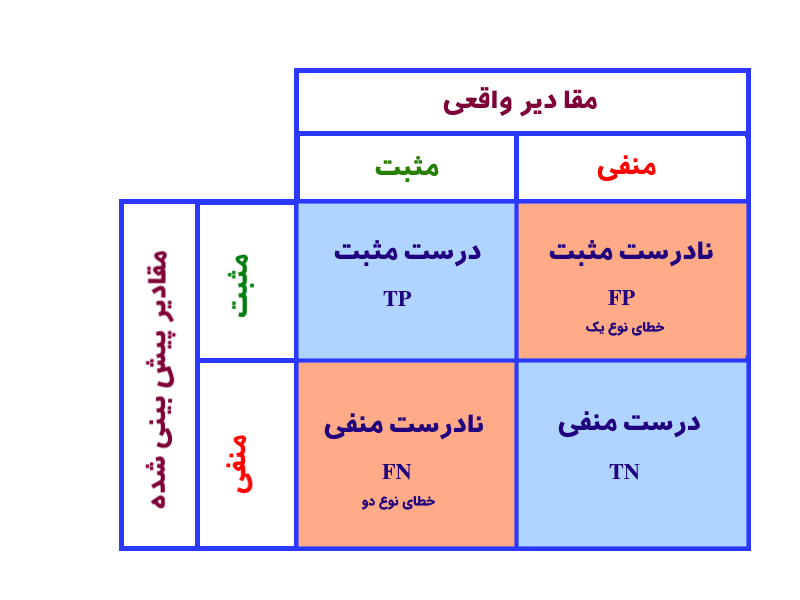
\includegraphics[height=8cm,width=10cm]{./confusion/Actual_Predicted.png}
   \caption{ ماتریس درهم‌ریختگی برای مسئله با دو دسته}
   \label{Confusion}
   \centering
\end{figure}

دقت: این معیار بیانگر دقت کل طبقه‌بندی است و بیانگر نرخ طبقه‌بندی صحیح است. همان‌طور که در رابطه \ref{eq:accuracy} مشاهده می‌شود. تمامی مفاهیم فوق در این رابطه اثر گذارند.

\begin{equation}
    \label{eq:accuracy}
    \text{Accuracy} = \frac{TP+TN}{TP+TN+FP+FN}
\end{equation}




خطا: از این معیار در کنار معیارهای دیگر استفاده می‌شود و بیانگر مقدار فاصله از مقادیر واقعی هر نمونه برای پیش‌بینی توسط مدل است. در رابطه \ref{eq:loss} نماد M بیانگر تعداد کلاس‌ها است و log لگاریتم طبیعی است.  $y_{o,c}$ یک نشانگر دودویی (0 یا 1) است اگر برچسب کلاس c طبقه‌بندی صحیح برای مشاهده o باشد ( برچسب‌های از قبل دانسته) و $p_{o,c}$ احتمال پیش‌بینی شده‌ای است که مشاهده o از کلاس c باشد (برچسب های پیش‌بینی).

\begin{equation} 
\label{eq:loss} 
\text{Loss}=-\sum_{c=1}^My_{o,c}\log(p_{o,c}) 
\end{equation}

\section{نتایج به‌دست آمده}

در ادامه به تاثیر دو پارامتر تعداد کارگران و تعداد دور‌های آموزشی بر هر یک از معیار‌های دقت و خطای کل مدل شبکه عصبی فرآیند یادگیری فدرال پرداخته شده است. به عنوان نمونه در این شبیه‌سازی یک‌ بار با ۱۰ کارگر و بار دیگر با ۵ کارگر اجرا شده است. لازم به ذکر است که نتایج آورده شده حالت محدودی از یک سناریو واقعی اینترنت اشیاء است که میتواند گاهاً تا هزاران دستگاه کم توان روی شبکه را نیز در بر بگیرد. در این آزمایش به دلیل کمبود منابع سخت افزاری و زمانی این تعداد را به اندازه یک شبکه داخلی (مثلا خانه هوشمند) محدود شده‌ است. طبق \cite{b12} میانگین تعداد این دستگاه‌ها در کشور ژاپن در هر خانه برابر با ۱۰.۳ عدد است که باتوجه کمتر بودن این عدد در کشور ایران، یکبار با ۷ عدد و بار دیگر با ۱۰ عدد شبیه ‌سازی شده است. در ادامه نمودار‌های مرتبط با نتایج این شبیه‌سازی در تصاویر \ref{ acc } و \ref{ loss } برای شهود بیشتر و بهتر آورده شده است.

\begin{figure}[H]
    \centering
   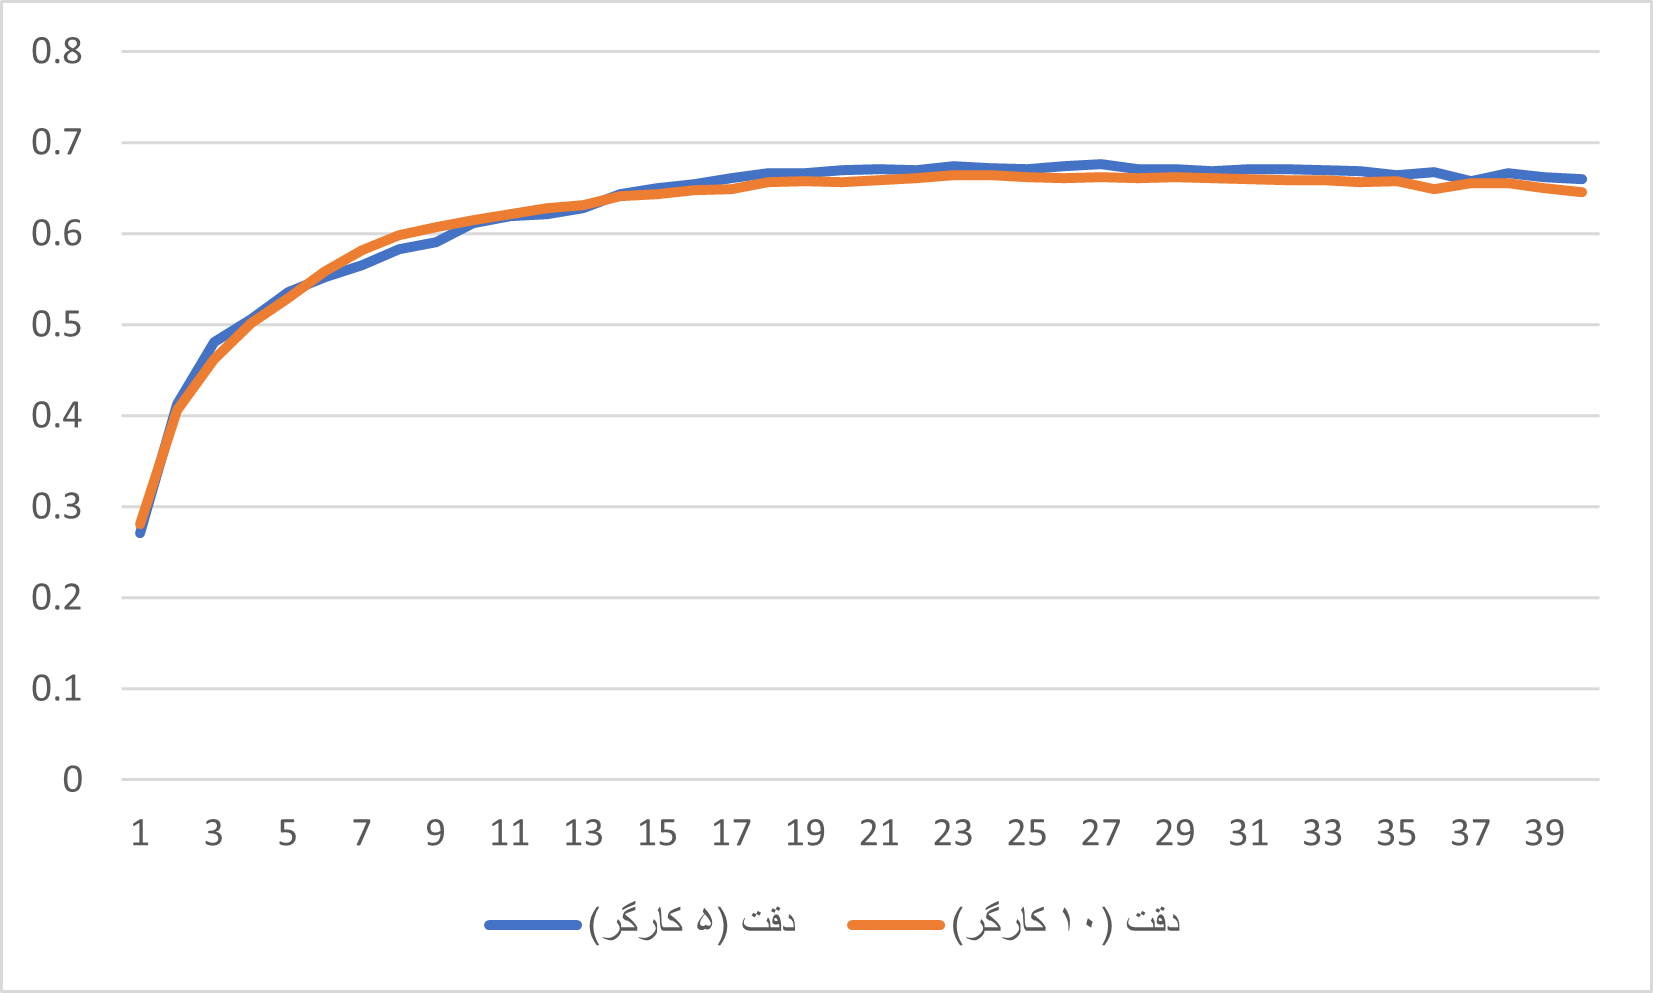
\includegraphics[height=10cm,width=14cm]{./charts/acc.png}
   \caption{ نمودار دقت به‌دست آمده در هر دور از آموزش سراسری}
   \label{ acc }
   \centering
\end{figure}

\begin{figure}[H]
    \centering
   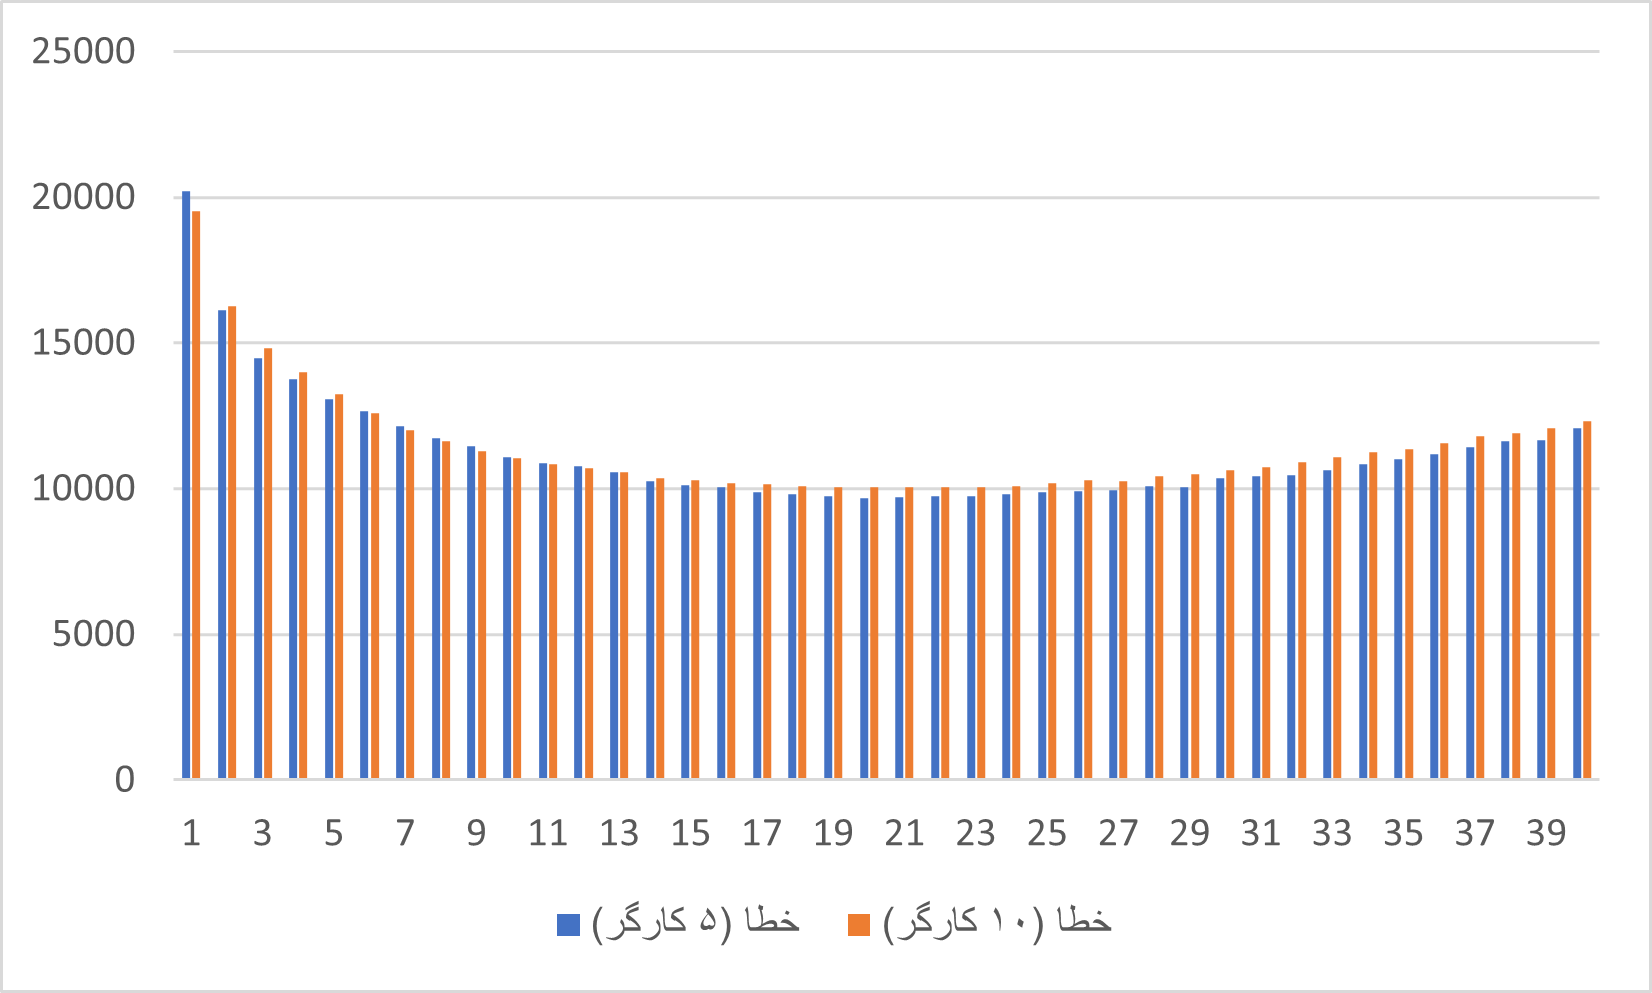
\includegraphics[height=10cm,width=14cm]{./charts/loss.png}
   \caption{ نمودار خطا در هر دور از آموزش سراسری }
   \label{ loss }
   \centering
\end{figure}

همان‌طور که از نمودار‌ها مشخص است، فرآیند آموزش در ابتدا سرعت بالایی دارد و در ادامه به یک خط مماس با شیب نسبتاً کم همگرا می‌شود تا در نهایت به صفر میل کند. با توجه به اینکه این فرآیند دو بار و با تعداد کارگران مختلف انجام شده است، می‌توان دید که تعداد دور آموزشی رابطه مستقیم بیشتری با تعداد کارگران دارد. البته اگر از یک استراتژی داینامیک به جای FedAVG استفاده شود، توقع داریم که به دقت‌های بالاتری برسیم و حتی سرعت همگرایی نیز با شیب بیشتری طی شود.

نمودار دوم گویای این است که طی یک روند غیرخطی در دور ۱۹ام به نقطه کمینه از نظر خطای مدل دسته‌بندی کننده می‌رسیم و در ادامه این روند رو به افزایش است. این می‌تواند بیانگر این باشد که آموزش بیشتر باعث می‌شود شبکه عصبی استفاده شده به عنوان مدل، رو به بیش برازش\LTRfootnote{Overfitting} شدن برود. همان‌طور که می‌دانیم ذات شبکه عصبی با آموزش زیاد به شدت مستعد بیش‌برازش شدن است. در \cite{bookG} روش‌هایی آورده شده تا با این‌ گونه رفتار مقابله شود.

نکته حائز اهمیت در این شبیه‌سازی این است که زمان تقریبی این شبیه‌سازی با ۱۰ کارگر در ۴۰ دور حدوداً ۴۵ دقیقه می‌باشد که زمان نسبتاً کمی در مقایسه با ماهیت یادگیری فدرال دارد. طبیعتاً در پیاده‌سازی‌های واقعی در شبکه‌های اینترنت اشیاء این زمان نمایی افزایش پیدا می‌کند.

\section{ پیشنهادها برای آینده}

همان‌طور که مشاهده شد، با قرار دادن یک لایه اضافه‌تر انتزاع\LTRfootnote{Abstraction} تحت عنوان لایه پردازش لبه در شبکه‌های اینترنت اشیاء‌ای که از یادگیری فدرال برای پیش‌بردن اهداف مدیرتی و تصمیم‌گیری خود استفاده می‌کنند، می‌توان کنترل و انعطاف‌پذیری بیشتری به شبکه داد. همان‌طور که دیده‌ شد، اضافه شدن این لایه به دلیل اینکه در دقت و کیفیت مدل استفاده شده داخل فرآیند یادگیری نسبت به عدم وجود آن حداقل پس‌رفتی به وجود نمی‌آورد و امید داریم که بهتر از قبل هم باشد، یک کار ارزشمند است. همچنین با اضافه شدن سرور لبه به سیستم یادگیری فدرال، دست برنامه‌نویسان نرم‌افزار نیز برای توسعه برنامه‌های کاربردی روی این شبکه‌ها به مراتب بازتر است.


اگرچه چندین راه حل تحقیقاتی برای کاهش چالش‌های اجرای یک سناریو خاص یادگیری فدرال  در شبکه شامل دستگاه‌های پردازش لبه پیشنهاد شده است، اما هنوز چالش‌هایی وجود دارد که حل نشده‌اند. علاوه بر ابتکارات تحقیقاتی گزارش شده در قسمت‌‌های قبلی، ایده‌های نوین قابل بحثی وجود دارند که در زیر توضیح داده شده است:
 
• فرآیند آموزش یادگیری فدرال با پشتیبانی چند مدل: در فرآیند آموزش یادگیری فدرال، فرض می‌شود که کارگران شرکت‌کننده پارامترهای مدل متناظر خود را با توجه به یک مدل سراسری به‌روز می‌کنند. با این حال، ممکن است کارگران بخواهند چندین مدل را حتی در زمان بطالت خود آموزش دهند؛ بنابراین، جداسازی جمع‌آوری مدل سراسری از آموزش محلی به کارگران اجازه می‌دهد تا از الگوریتم‌های یادگیری مختلف استفاده کنند. به عنوان مثال، ممکن است لازم باشد هم‌زمان چندین مدل مختلف با استفاده از روش فدرال برای اهداف مختلف توسعه یابند؛ بنابراین، تکنولوژی‌های مناسب بایستى تجزیه و تحلیل و پیاده‌سازی شود.
 
• تأثیر کانال شبکه بى‌سیم: دستگاه‌های لبه اغلب از طریق کانال‌های بی‌سیم به سرویس‌دهنده‌های لبه یا ابرى وصل شده‌اند؛ بنابراین، بررسى تأثیر الزامات شبکه، به ویژۀ ارتباطات بی‌سیم، در دقت آموزش مدل فدرال به‌عنوان یک روند تحقیقاتى آینده در نظر گرفتۀ شده است. نویز، خسارت مسیر، ترافیک بالا و قطعی همۀ نقص‌هایی هستند که بایستى در سیستم‌های ارتباطات بی‌سیم در نظر گرفتۀ شود. باید توجه داشت که در سناریو‌های اینترنت اشیاء نیز قطع و وصل شدن دستگاه‌های انتهایی خود دلیلی محکم بر این تأثیرات مخرب می‌باشد.

• انتخاب پویای کارگران و جمع‌آوری تطبیقى مدل: جمع‌آوری مدل تطبیقى و انتخاب مشترى پویا برای تخصیص منابع با در نظر گرفتن رفتار ناهمگون داده، قدرت محاسباتى، اندازۀ داده، ظرفیت شبکه و قابلیت اطمینان لینک در بین کارهای تحقیقاتى آینده قرار دارد. بنابراین، بایستى به‌ عنوان روندهای تحقیقاتی آینده، انتخاب پویای کارگران و جمع‌آوری تطبیقى مدل را بررسى کرد. به ‌عنوان ‌مثال، الگوریتم‌ها و پیچیدگی‌های مناسب برای درخواست‌های پویا کارگر و منابع ناهمگون در هر دو سمت کارگر و سرور اصلی دهنده. در چنین سناریوهایی، باید بتوان فرآیند آموزش یادگیری فدرال را مدیریت کرد. یکی از ایده‌های تعیین ضرایب و پارامتر‌ها برای انتخاب پویا کارگران و جمع‌آوری تطبیقى مدل، تخمین‌زدن تقریبی و تنظیم آن در سرور لبه می‌باشد. این محل که در مرکز شبکه اینترنت اشیاء قرار دارد، تخمین خوبی از رفتار کلی شبکه در اختیار الگوریتم‌های تنظیم‌کننده پارامتر‌ها قرار می‌دهد\cite{a13}.

• روش جدید یادگیری فدرال: اندازه مدل یادگیری فدرال بسیار بزرگ است تا بتواند در یک دستگاه لبه با منابع محدود جا شود. علاوه بر این، آموزش مدل یادگیری فدرال بسیار کند است و نمی‌تواند به همگرایى برسد و نیازهای تأخیر در برخى از برنامه‌های حساس به تأخیر را برآورده کند. روش جدید یادگیری فدرال موردنیاز است تا به طور پویا اهداف را دستیابی کند؛ بنابراین، یادگیرى فدرال پویا و تطبیقى بایستى برای دستگاه‌های لبه با منابع محدود تجزیه و تحلیل و پیاده سازى شود. به عنوان مثال میتوان با وزن دادن به گره‌ها در الگوریتم FedAVG و میانگین وزن‌دار گرفتن از آن‌ها در حین اجرای سیستم، به دقت و سرعت بالاتری دست پیدا کرد.

• پیاده‌سازی پروتکل‌های پیچیده به‌منظور بهبود کیفیت ارتباطات در فرآیند یادگیری: می‌توان از پروتکل‌های مختلف که بعضی سنگین و بعضی دیگر سبک هستند به‌منظور ایجاد یک پروسه یادگیری امن و مطلوب در بستر شبکه استفاده کرد. پیاده‌سازی این پروتکل‌ها می‌تواند معطوف به دستگاه‌های انتهایی نباشد و سرور لبه نیز در آن نقش مشخصی داشته باشد. یکی از این پروتکل‌ها که بدون در نظر گرفتن سرور لبه توسعه پیدا کرده پروتکل SAFA\LTRfootnote{Semi-Asynchronous Protocol for Fast Federated Learning with Low Overhead} است که ساختاری وابسته به حالت\LTRfootnote{Stateful} ارائه می‌کند که باعث افزایش سرعت همگرایی می‌شود. در واقع با دسته‌بندی کارگران و نگه داشتن وضعیت اخیر آنها در پروسه یادگیری با دادن برچسب‌های مخصوصی به آنها و دسته‌بندی کردن آنان به هرکدام وظایف معینی می‌دهد. می‌توان با محدود کردن این پروتکل و اضافه کردن نقش سرور لبه به آن، به کار آن سرعت و دقت بیشتری بخشید\cite{SAFA}.

• امنیت بالاتر با استفاده از سرور لبه: از دانش قبلی می‌دانیم که یکی از بنیادی‌ترین دلایل به وجود آمدن یادگیری فدرال امنیت بالای آن در مقایسه با دیگر روش‌های یادگیری توزیع شده است. اما روش‌های جدیدی آمده که با داشتن دیتای مربوط به کارگران و سرور تجمیع کننده و شنود کردن این داده‌ها روی شبکه به روش‌های مرسوم مانند جعل آدرس\LTRfootnote{Spoofing} و بررسی ترافیک شبکه\LTRfootnote{Sniffing}، می‌توان طی چند دور به مدل داخل سرور اصلی تا حد خوبی دست پیدا کرد\cite{n2}. با اضافه کردن یک سرور لبه برای افزایش ایمنی، می‌توان از این راهکار جلوگیری کرد و این روند را سخت‌تر و طولانی‌تر کرد.
%%%%%%%%%%%%%%%%%%%%%%%%%%%%%


% Appendices
\appendix
%% Appendix 1
\chapter{الگوریتم FedAVG }

از مطرح‌ترین و ساده‌ترین روش‌های ادغام کردن پارامتر‌های ارسالی (به عنوان مثال وزن‌ها و بایاس‌های شبکه عصبی) توسط تجمیع کننده الگوریتم میان‌گیری از آن‌ها با وزن یکسان بین تمامی کارگران می‌باشد. این الگوریتم با نام \lr{Federated Averaging} برای اولین بار در \cite{b6} مطرح شده است. در نسخه‌های اولیه یادگیری فدرال، این الگوریتم به صورت متمرکز درون تجمیع کننده در انتهای هر دور از یادگیری اجرا می‌شود تا در نهایت تمام کارگران با وزن یکسان در فرآیند یادگیری سهیم باشند. در ادامه شبه‌کد دو تکه اصلی مورد نیاز از اجرای این الگوریتم در تجمیع‌کننده و کارگران آورده شده است.


از مهم‌ترین ایراداتی که می‌توان به این نوع الگوریتم گرفت این است که به علت ناهمگونی داده‌ها بین کارگران نباید در میانگین‌گیری وزن یکسانی به آنها داد. به همین دلیل طی سال‌های اخیرمدل‌های پیشرفته‌تری از این استراتژی معرفی شده است\cite{ref4}.


\begin{algorithm}[tbp]
    \caption{بروزرسانی مشترک: اجرا در هر کارگر}
    \label{alg:client_update}
    \begin{algorithmic}[1]
        \State \textbf{ورودی:} بردار وزن مدل $w$، (\lr{Local Mini Batch})اندازه دسته‌های کوچک محلی $B$
        \State \textbf{خروجی:} بردار وزن مدل به‌روزشده $w'$
        
        \Function{بروزرسانی-مشترک}{$w, B$}
            \State تقسیم $P_k$ به دسته‌هایی به اندازه $B$: $بچها \gets \text{تقسیم\_به\_بچها}(P_k, B)$
            
            \For{$i = 1$ تا $E$} \Comment{عبورهای آموزشی محلی}
                \For{$هر دسته$ در $دسته‌ها$}
                    \State $w \gets w - \eta \cdot \nabla f(w,دسته)$ \Comment{بروزرسانی وزن‌های مدل}
                \EndFor
            \EndFor
            
            \State \Return $w$
        \EndFunction
    \end{algorithmic}
\end{algorithm}

\begin{algorithm}[tbp]
    \caption{میانگین‌گیری مشترک: اجرا در سرور}
    \label{alg:federated_averaging}
    \begin{algorithmic}[1]
        \State \textbf{ورودی:} نرخ یادگیری جهانی $\eta$، تعداد کارگر‌ها در هر دور $C$، تعداد عبور آموزشی محلی $E$، اندازه مینی‌بچ محلی $B$
        \State \textbf{خروجی:} بردار وزن مدل میانگین $w_{\text{avg}}$
        
        \Function{میانگین‌گیری-مشترک}{$\eta, C, E, B$}
            \State مقداردهی اولیه بردار وزن مدل: $w \gets w_0$
            
            \For{$t = 1$ تا $\infty$} \Comment{دوره‌های آموزشی}
                \State انتخاب به صورت تصادفی $C$ کارگر: $کارگر‌های\_انتخاب‌شده \gets \text{انتخاب\_کارگر‌ها}(C)$
                
                \For{$k$ در $کارگر‌های\_انتخاب‌شده$}
                    \State انجام بروزرسانی مشترک برای کارگر $k$: $w_k \gets \text{بروزرسانی-مشترک}(w, B)$
                    \State بروزرسانی بردار وزن مدل برای کارگر $k$: $w \gets \text{تجمیع\_وزن‌ها}(w, w_k)$
                \EndFor
                
                \State محاسبه میانگین وزن‌های تمام کارگر‌ها: $w_{\text{avg}} \gets \text{محاسبه\_میانگین\_وزن‌ها}(w, C)$
            \EndFor
            
            \State \Return $w_{\text{avg}}$
        \EndFunction
    \end{algorithmic}
\end{algorithm}


% Appendix 2
\chapter{پروتکل SAFA }

یکی از پروتکل‌هایی که قابلیت پیاده‌سازی برای فرآیند یادگیری فدرال دارد، پروتکل SAFA است. همان‌طور که در شکل \ref{SAFA} مشهود است، این پروتکل با دسته‌بندی کارگران به ۳ دسته انتخاب شده\LTRfootnote{Picked Client}، تعیین نشده\LTRfootnote{Undrafted Client} و قطع شده\LTRfootnote{Crashed Client} تقسیم می‌کند. این دسته بندی با توجه به نحوه برقراری ارتباط با کارگر در دورهای قبلی هست که در کش ذخیره می‌شود. پروتکل SAFA با استفاده از یک الگوریتم تصادفی، تعدادی از کارگران را به عنوان انتخاب شده انتخاب می‌کند و به آن‌ها دستور می‌دهد که مدل خود را به سرور ارسال کنند. سپس، سرور با دریافت مدل‌های ارسال شده، آن‌ها را با هم ترکیب می‌کند و مدل جدید را به کارگران انتخاب شده برمی‌گرداند. در صورتی که یک کارگر در یک دوره از ارسال یا دریافت مدل عقب بماند، به عنوان قطع شده در نظر گرفته می‌شود و در دوره‌های بعدی حذف می‌شود. همچنین، در صورتی که یک کارگر به طور مکرر در دوره‌های مختلف انتخاب نشود، به عنوان تعیین نشده شناخته می‌شود و احتمال انتخاب آن در دوره‌های آینده کاهش می‌یابد. پروتکل SAFA با استفاده از این روش، سعی دارد تا تعادل بین سرعت و دقت فرآیند یادگیری فدرال را حفظ کند\cite{SAFA}.


\begin{figure}[H]
    \centering
   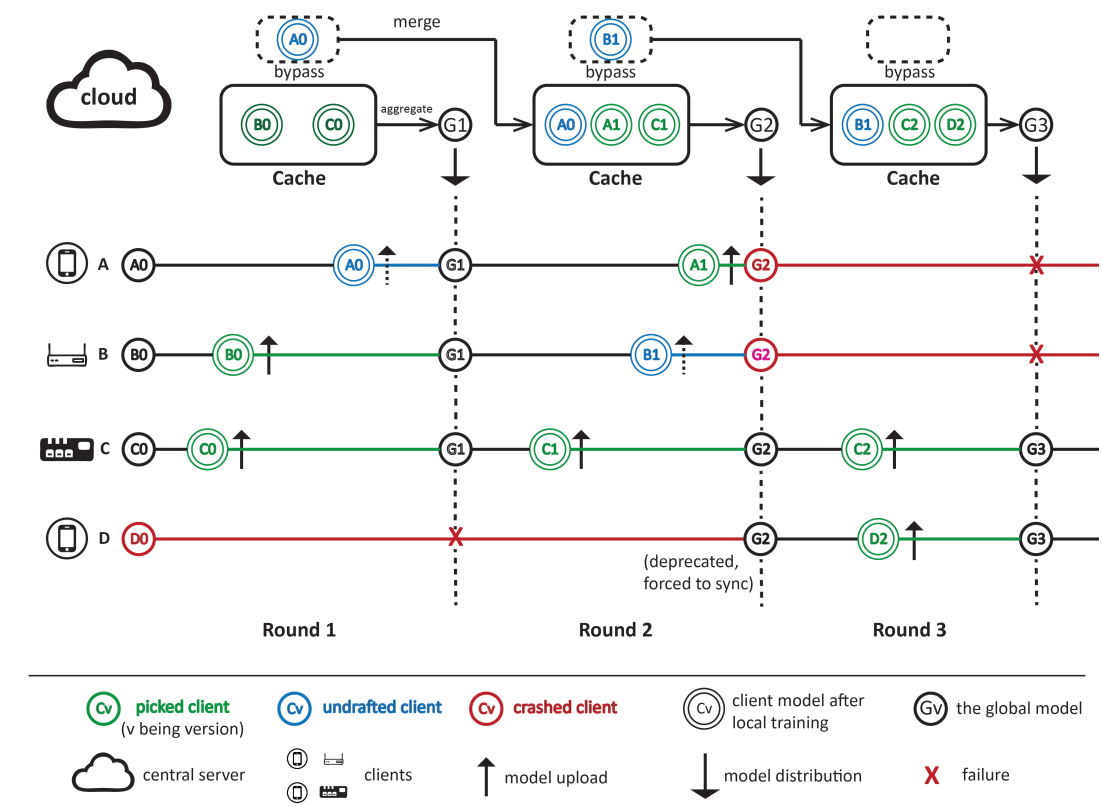
\includegraphics[height=12cm,width=14cm]{./SAFA/ex.png}
   \caption[سناریو‌ای از اجرای پروتکل SAFA در ۳ دور]{ سناریو‌ای از اجرای پروتکل SAFA در ۳ دور\cite{SAFA} }
   \label{SAFA}
   \centering
\end{figure}

با توجه به شکل، کش مدل‌های محلی آخرین کارگر‌های انتخاب شده را که برای تجمیع استفاده می‌شوند، نگه می‌دارد. کارگر‌هایی که نتایج آن‌ها انتخاب نشده‌اند، کارگر‌های رد شده هستند (با رنگ آبی)، مثلاً کارگر A در دور 1 و کارگر B در دور 2.به‌روزرسانی‌های این کارگر‌ها در ساختار میان‌بر\LTRfootnote{Bypass} ذخیره می‌شوند تا از کار بیهوده در سمت محلی جلوگیری شود. کارگر‌هایی که به هر دلیلی (مثل خروج از برنامه یا قطع شدن اینترنت) نمی‌توانند آموزش محلی خود را تکمیل کنند، کارگر‌های خراب هستند (با رنگ قرمز برجسته شده)، مثلاً کارگر D در دور 1. کارگر‌هایی که به‌روزرسانی‌های آن‌ها انتخاب شده‌اند، کارگر‌های انتخاب شده نامیده می‌شوند (با رنگ سبز)، مثلاً کارگر B و C در دور 1.


توزیع مدل با تحمل تأخیر\LTRfootnote{Model Distribution With Lag Tolerance}: در این مرحله، سرور مدل خود را به کارگران مختلف ارسال می‌کند و از آن‌ها می‌خواهد که بر روی داده‌های خود به روزرسانی مدل را انجام دهند. سرور همچنین یک حداکثر زمان تأخیر را برای دریافت مدل‌های به روز شده تعیین می‌کند. این روش اجازه می‌دهد که کارگران با سرعت‌های مختلف و با تأخیرهای متفاوت در فرآیند یادگیری شرکت کنند.

اولین رسیدن برابر است با اولین ادغام\LTRfootnote{First Come First Merge}: در این مرحله، سرور با دریافت مدل‌های به روز شده از کارگران، آن‌ها را با هم ترکیب می‌کند. سرور برای ترکیب کردن مدل‌ها، از الگوریتم «اولین رسید، اولین ترکیب شد» استفاده می‌کند. این الگوریتم به این صورت است که سرور همواره یک نسخه از مدل را نگه دارد و هر گاه یک مدل جدید از یک کارگر دریافت کند، آن را با نسخه فعلی ترکیب کرده و نسخه جدید را ذخیره می‌کند.

تجمیع تمایزدهنده\LTRfootnote{Discriminative Aggregation}: در این مرحله، سرور با استفاده از یک الگوریتم تجمیع تمایزدهنده، مقادیر وزن‌های مختلف در مدل را با هم مقایسه کرده و آن‌ها را به صورت چند جمله‌ای درجه دو نمایش می‌دهد. سپس، با استفاده از چند جمله‌ای حاصل، سطح خطای هر وزن را برآورد کرده و وزن‌های با خطای بالاتر را حذف یا کم کاربرد می‌کند. این روش باعث بهبود دقت و کارآمدی فرآیند یادگیری فدرال می‌شود.

باتوجه به کاربرد‌های متنوع این پروتکل و قابلیت انعطاف بالا خصوصاً زمانی که دستگاه‌های کارگر از سخت‌افزارهای ناهمگون بهره ببرند می‌تواند به‌شدت فرآیند یادگیری را تسریع کند.



% References
\renewcommand{\bibname}{مراجع}
\addcontentsline{toc}{chapter}{مراجع}

\begin{thebibliography}{99}

\begin{latin}

\baselineskip=.7cm

\bibitem{b7}
E. Baccour et al., "Pervasive AI for IoT Applications: A Survey on Resource-Efficient Distributed Artificial Intelligence," in \textit{IEEE Communications Surveys and Tutorials}, vol. 24, no. 4, pp. 2366-2418, Fourthquarter 2022, doi: 10.1109/COMST.2022.3200740.

\bibitem{b8}
A. A. Osuwa, E. B. Ekhoragbon and L. T. Fat, "Application of artificial intelligence in Internet of Things," in \textit{2017 9th International Conference on Computational Intelligence and Communication Networks (CICN)}, Girne, Northern Cyprus, 2017, pp. 169-173, doi: 10.1109/CICN.2017.8319379.

\bibitem{a10}
Dinh C. Nguyen, Ming Ding, Pubudu N. Pathirana, Aruna Seneviratne, “Federated Learning for Internet of Things:
A Comprehensive Survey”,\textit{arXiv:2104.07914v1}, 2021.

\bibitem{book_1}
Kairouz, P., McMahan, H.B., Avent, B., Bellet, A., Bennis, M., Bhagoji, A.N., Bonawitz,
K., Charles, Z., Cormode, G., and Cummings, R., “Advances and open problems in federated
learning”, \textit{Foundations and Trends® in Machine Learning}, vol. 14, no. 1–2, pp. 1-210, 2021.

\bibitem{b6}
\noindent H. Brendan McMahan, Eider Moore, Daniel Ramage, Seth Hampson, Blaise Aguera y Arcas, “Communication-Efficient Learning of Deep Networks from Decentralized Data” \textit{AISTATS}, Google, Inc., 2017.

\bibitem{b1}
Beutel, Daniel J and Topal, Taner and Mathur, Akhil and Qiu, Xinchi and Fernandez-Marques, Javier and Gao, Yan and Sani, Lorenzo and Kwing, Hei Li and Parcollet, Titouan and Gusmão, Pedro PB de and Lane, Nicholas D, “Flower: A Friendly Federated Learning Research Framework” \textit{arXiv preprint arXiv:2007.14390}
, 2020.

\bibitem{a1} 
Wang, Xingwei and Zhao, Hong and Zhu, Jiakeng, “GRPC: a communication cooperation mehanism in distributed systems”,  \textit{Association for Computing Machinery}, 1993.

\bibitem{b9} 
M. Galar, A. Fernández, E. Barrenechea, H. Bustince, F. Herrera, “An overview of ensemble methods for binary classifiers in multi-class problems: Experimental study on one-vs-one and one-vs-all schemes,” in \textit{Pattern Recognition}, vol. 44, no. 8, pp. 1761-1776, August 2011, Elsevier.

\bibitem{a11}
Liu, Yang and Fan, Tao and Chen, Tianjian and Xu, Qian and Yang, Qiang, “FATE: An Industrial Grade Platform for Collaborative Learning with Data Protection
”,\textit{JMLR.org}, 2021.

\bibitem{b12}
 J. Koetsier, “Smart Home: Apple Is The Fastest-Growing Connected Device Company,” Forbes, Aug 31, 2022

\bibitem{bookG} 
J. Brownlee, “Better Deep Learning: Train Faster, Reduce Overfitting, and Make Better Predictions,” Machine Learning Mastery, December 13, 2018.

\bibitem{a13} 
 Portnoy, A., Tirosh, Y., Hendler, D., “Towards Federated Learning With Byzantine-Robust Client Weighting”, \textit{arXiv:2004.04986v2}, 2021

\bibitem{SAFA}
Wentai Wu, Ligang He, Weiwei Lin, Rui Mao, Carsten Maple, Stephen Jarvis, “SAFA: a Semi-Asynchronous Protocol for Fast Federated Learning with Low Overhead”,
 \textit{arXiv:1910.01355v4}, v. 4, 2021.

\bibitem{n2} 
Geiping, J., Bauermeister, H., Dröge, H., Moeller, M., “Inverting Gradients – How easy is it to break privacy in federated learning?”, \textit{arXiv:2003.14053v2}, 2020

\bibitem{paper_4}
Mahmod, Ahmad and Caliciuri, Giuseppe and Pace, Pasquale and Iera, Antonio, ``Improving the Quality of Federated Learning Processes via Software Defined Networking", \textit{Association for Computing Machinery}, 2023.


\bibitem{edge1}
Abreha, Haftay Gebreslasie, Mohammad Hayajneh, and Mohamed Adel Serhani, "Federated Learning in Edge Computing: A Systematic Survey",\textit{Wireless Sensor Networks towards the Internet of Things}, Sensors 22, no. 2: 450 , 2022

\bibitem{edge2}
Dhurgham Hassan Mahlool, Mohammed Hamzah Abed, "A Comprehensive Survey on Federated Learning: Concept and Applications",\textit{Computer Vision and Pattern Recognition}, arXiv:2201.09384 , 2022

\bibitem{ref5} 
Tuo Zhang, Lei Gao, Chaoyang He, Mi Zhang, Bhaskar Krishnamachari, Salman Avestimehr, “Federated Learning for Internet of Things: Applications, Challenges, and Opportunities”, \textit{arXiv:2111.07494v4}, v. 4, 2022.

\bibitem{ref6}
 Zhi Zhou, Xu Chen, En Li, Liekang Zeng, Ke Luo, Junshan Zhang, “Edge Intelligence: Paving the Last Mile of Artificial Intelligence with Edge Computing”, \textit{arXiv:1905.10083v1}, v. 1, 2019.

\bibitem{ref7} 
 Andy Chen and Chaitanya Asawa, “Going beyond the bounding box with semantic segmentation”, \textit{The Gradient}, 2018.

\bibitem{ref8} 
Zewen Li, Wenjie Yang, Shouheng Peng, Fan Liu, “A Survey of Convolutional Neural Networks: Analysis, Applications, and Prospects”, \textit{arXiv:2004.02806v1}, v. 1, 2020.

\end{latin}



\bibitem{ref3}
طلائي مهتاب "	توسعه‌ي الگوريتم و بررسي عملكرد يادگيري پراكنده با حريم شخصي تفاضلي تطبيقي``، \textit{استقلال،} دانشگاه صنعتی اصفهان، شماره~۱۷۷۵۸، صص~27-34، ۱۴۰۱.

\bibitem{ref4} 
 بزرگ‌زاد علی, “بررسی روشهای حل مشکل ناهمگونی آماری در یادگیری فدرال”, \textit{سمینار کارشناسی ارشد هوش مصنوعی و رباتیکز}, دانشگاه صنعتی اصفهان, 1401. 

\end{thebibliography}



\addcontentsline{toc}{chapter}{چکیده انگلیسی}
\thispagestyle{empty}

\begin{latin}
\begin{center}

{\Huge Edge Computing Empowers Federated Learning in Resource-Constrained IoT Networks}

\vspace{1cm}

{\LARGE{Amirreza Hosseini}}

\vspace{0.2cm}

{\small amirreza.hosseini@ec.iut.ac.ir}

\vspace{0.5cm}

September 2023

\vspace{0.5cm}

Department of Electrical and Computer Engineering

\vspace{0.2cm}

Isfahan University of Technology, Isfahan 84156-83111, Iran

\vspace{0.2cm}

Degree: B.Sc. \hspace*{3cm} Language: Farsi

\vspace{1cm}

{\small\textbf{Supervisor: Dr. Amir Khorsandi (khorsandi@iut.ac.ir)}}
\end{center}
~\vfill



\noindent\textbf{Abstract}

\begin{small}
\baselineskip=0.6cm
Artificial Intelligence (AI) has rapidly expanded into various fields in recent years, becoming a fundamental technology in numerous applications. To meet the diverse needs of these applications, various approaches and methods have been proposed to achieve the infrastructure related to AI technology. One of these methods is the Machine Learning (ML) approach for privacy preservation, known as Federated Learning (FL). FL enables the development of applications that perform analysis and AI-based services on sensitive user data while complying with strict privacy regulations in various domains, including healthcare, finance, and transportation, particularly the Internet of Things (IoT).
It is worth noting that FL can be executed on a large number of heterogeneous final devices, which are typically distributed and have limited processing power and energy resources. This presents a significant challenge that can hinder the effective, sustainable, and scalable execution of FL.

To address these challenges, recent research has proposed the use of edge computing in FL. Edge computing involves using the storage, communication, and computing capabilities of edge servers located near end devices to reduce system latency. Performing primary computations and preprocessing close to the data source can reduce the amount of traffic sent to the main server and decrease access delays. This approach can also be effective in improving the performance of FL, which is the main focus of this project.

Therefore, the objective of this project is to propose a structure that provides a suitable platform for developing FL in networks with edge computing capabilities. The proposed structure aims to address the challenges of executing FL on heterogeneous and resource-constrained devices by leveraging the capabilities of edge servers. The resulting system improves the performance and scalability of FL while complying with strict privacy regulations.

\end{small}

\vspace{0.5 cm}

\noindent \textbf{Key Words}: Federated learning, Internet of Things, Edge computing, Machine Learning, Artificial Intelligence

\end{latin}

%********************************
% Page before last: English Signatures
%********************************
\thispagestyle{empty}
\newgeometry{left=3cm,right=3cm,top=2cm}
% \begin{latin}
% \begin{center}
% 
\includegraphics[height=3cm]{iut_logo.png}
% \vspace{0.4cm}

% {\large\textbf{Isfahan University of Technology}}\\

% \vspace{0.4cm}
% Department of Electrical and Computer Engineering

% \vspace{2.5cm}

% {\Huge Increasing Efficiency in Low-Efficiency Systems}

% \vspace{1.5cm}

% {\large
% 	A Thesis
	
% 	\vspace{.3cm}
	
% 	Submitted in partial fulfillment of the requirements
	
% 	\vspace{.3cm}
	
% 	for the degree of Master of Science
% }

% 	\vspace{1.5cm}

% {\Large
% 	\textbf{by}
	
% 	\vspace{.3cm}
	
% 	\textbf{Azin Azadeh}
% }
% \end{center}

% \vfill

% Evaluated and Approved by the Thesis Committee, on March 21, 2015
% \vspace{0.5cm}

% \begin{enumerate}
% \item Bahram Borzou, Prof. (Supervisor)
% \vspace{0.5cm}

% \item Poorya Parniani, Assoc. Prof. (Advisor)
% \vspace{0.5cm}

% \item Tahamtan Trabi, Prof. (Examiner)
% \vspace{0.5cm}

% \item Soraya Sanaei, Assist. Prof (Examiner)
% \vspace{0.5cm}

% \end{enumerate}

% Jamshid Jahangir, Department Graduate Coordinator

% \pagebreak
% \end{latin}

%***************************
% last page: Blank
%***************************
\thispagestyle{empty}
\mbox{}

% It's finally over. Wasn't that hard, was it?

\end{document}